\chapter{Frequency Dynamics in Sinusoidal Neural Networks}
\label{chap:sinusoidal}

In this chapter, we explore the frequency dynamics within sinusoidal neural networks, laying the groundwork for designing architectures that can represent signals across multiple resolutions. While much of the research on sinusoidal neural networks has focused on their capacity to capture high-frequency details, the interplay between frequency initialization, network structure, and learned representations is still not fully understood. Our goal is to analyze these factors systematically and establish a deeper understanding of how frequency components propagate and interact in both shallow and deep sinusoidal architectures.

We begin by studying simple, one-dimensional signals and progressively increase the complexity of our experiments to evaluate how different initializations and network capacities affect frequency learning. Through a series of controlled experiments, we demonstrate how the number of neurons, the inclusion of hidden layers, and specific initialization parameters impact the networks' ability to isolate and reconstruct frequency bands. We also address the phenomenon of capacity-based filtering, highlighting how network size and depth influence the learned signal spectrum. These findings are essential in preparing for more sophisticated architectures, where multiresolution properties and frequency control become the key elements in building neural representations for complex media.

We initially focus on representing one-dimensional signals using sinusoidal neural networks. This approach allows us to experiment on the control of signal frequencies, visualize them through their Fast Fourier Transform (FFT) plots, and validate our results against classical sampling theory.Our architecture builds upon the Sinusoidal Representation Networks (SIREN) framework (\cite{sitzmann2019siren}), known for its ability to learn high-frequency signal details efficiently and model signal derivatives. We deeply investigate the network's initialization, exploring the interplay between its hyperparameters, the inherent frequencies of a signal, and the frequencies the network learns.



\section{Related Works}

Our focus lies on signals as media objects, usually represented by functions in one, two, and three dimensions. \cite{tancik2020fourfeat} demonstrated, both theoretically and empirically, that standard Multilayer Perceptrons (MLPs) struggle to learn high frequencies in such domains, which are considered low-dimensional domains for machine learning applications. They proposed using Fourier feature mapping to transform input coordinates into a higher-dimensional spectral feature space before processing them through the network. This enables coordinate-based MLPs to effectively capture high-frequency content in low-dimensional signals, overcoming this \textit{spectral bias} (\cite{rahaman2018spectral}).

Sinusoidal neural networks represent a class of coordinate-based networks that employs the sine function as their activation function. They serve as a bridge between spatial and spectral domains due to the close relationship between the sine function and the Fourier basis. The first layer of a sinusoidal neural network projects the signal into spectral space, while the last layer reconstructs the signal from a dictionary of spectral atoms. This characteristic allows them to naturally overcome the spectral bias of regular MLPs. However, these sinusoidal neural networks have been regarded as difficult to train \cite{taming2017}. To address this issue, Sitzmann et al. \cite{sitzmann2019siren} proposed SIREN, a sinusoidal network for signal representation. One of its key contributions is an initialization scheme that ensures stability and convergence, enabling the modeling of fine details consistent with the signal’s frequency content.

The challenge in training sinusoidal neural networks comes in part from the composition of sinusoidal functions, which can generate multiple new and higher frequencies. \cite{novello2022understanding} studied sinusoidal MLPs by expanding them as harmonic sums, demonstrating how numerous new frequencies are expressed as integer linear combinations of the input frequencies. This work provides theoretical justification for sinusoidal MLPs compactness property and contributes to a better understanding of these networks’ behavior.

A simpler form of sinusoidal network is the Multiplicative Filter Network (MFN) \cite{fathony2020multiplicative}, which is equivalent to a shallow sinusoidal MLP. \cite{bacon2021} introduced the Band-Limited Coordinate Network (BACON), an MFN that produces intermediate outputs with an analytically specified spectral bandwidth, achieving multiresolution representations of underlying signals. While its structure allows BACON to be expressed as a linear combinations of sines, avoiding the composition of sines present in deep sinusoidal MLPs, it creates multiresolution representations by truncating the frequency spectra of the signals at a specific value. This approach produces ringing artifacts in some levels of detail, and becomes evident when we look at the Fourier transform of images reconstructed using this network (see Chapter \ref{ch:imaging}).

The ability to control frequency bands in representation is closely tied to the capability of adaptively reconstructing signals at multiple detail levels. \citet{mueller2022instant} developed a multiresolution neural network architecture based on hash encoding, while \citet{martel2021acorn} designed an adaptive coordinate network for neural signals.

In this context, we introduce \textit{Multiresolution Sinusoidal Neural Networks} (MR-Net) \cite{paz2022,paz2023mr} based on classical signal multiresolution representations. Our results in imaging applications, discussed in Chapter \ref{ch:imaging}, demonstrate that MR-Net outperforms the previous state-of-the-art technique, BACON, while utilizing a smaller number of parameters.


\section{Frequency Initialization}

The correct initialization of sinusoidal neural networks is crucial for having stability during training and convergence to the expected result. According to \cite{sitzmann2019siren}, a SIREN model must be initialized so that for a uniform input in $[-1, 1]$ the outputs of each hidden layer before the sine nonlinearity are standard normal distributed. 

Moreover, the authors of SIREN propose to initialize the first layer of the network so that the sine function $\sin(\omega_0 \cdot W x + b)$ spans multiple periods over $[-1, 1]$. They introduce $\omega_0$ as a hyperparameter that could be adjusted to each signal, while $W$ and $b$ are the weights and biases of a layer in the network. For the examples presented in their work, they used a fixed $\omega_0=30$ and found it to work well empirically, but they did not dive deeper on the \emph{why}.

% The authors of SIREN suggest initializing the first layer of the network to ensure that the sine function \(\sin(\omega_0 \cdot Wx + b)\) spans multiple periods over \([-1, 1]\). They introduce \(\omega_0\) as a hyperparameter that can be adjusted for each signal. Empirically, they found a fixed \(\omega_0 = 30\) to work well, although they do not delve into the underlying reasons.

% In this section, we show how the choice of $\omega_0$  impacts the frequencies learned by the network, the speed of the training and even if it will converge to a reasonable result or collapse into noise. The hyperparameter $\omega_0$ is directly related to the interval of frequencies used to initialize the first layer of the network, determining the set of the spectral atoms where the signal will be projected. This same hyperparameter is also applied on the initialization of the hidden layers as the authors argue it boosts the gradients during the training and accelerates the convergence. However, in the hidden layers, it is basically used as pre-conditioner, a numeral trick, since the implementation multiplies by $\omega_0$ and also divides by this same value. We propose to call this hyperparameter in the hidden layers by $\omega_h$, and keep $\omega_0$ only for the first layer.

In this section, we examine how the choice of \(\omega_0\) impacts the frequencies learned by the network, \red{the speed of training}, and whether the network will converge to a reasonable result or collapse into noise. We show that the hyperparameter \(\omega_0\) directly influences the range of frequencies used to initialize the first layer of the network, thus determining the set of spectral atoms onto which the signal will be projected. This hyperparameter is also applied to the initialization of the hidden layers, as the authors argue that it boosts gradients during training and accelerates convergence. However, in the hidden layers, \(\omega_0\) functions primarily as a pre-conditioner, a numerical trick, since the implementation multiplies the weights by \(\omega_0\) and then divides them by the same value. To clarify this distinction, we propose referring to the hyperparameter in the hidden layers as \(\omega_h\), reserving \(\omega_0\) exclusively for the first layer. In all experiments, the hyperparameter $\omega_h$ will be kept constant equal 30 unless explicitly stated on contrary.

By understanding and adjusting \(\omega_0\), we aim to optimize the training process of sinusoidal neural networks and develop a multiresolution architecture with them.


\subsection{Isolating Frequencies}

A shallow network with just one layer of sinusoidal activation functions can filter a signal by band-limiting its frequency content. Thus, it provides a tool for controlling the level of detail of the output signal. This conclusion is natural since the resulting signal representation is a linear combination of sinusoidal functions with induced frequency band. In a sense, the network is projecting the input signal into a learned dictionary of spectral atoms.

In that context, a one-layer SIREN network could also be used as a spectral filter, just as in the MFN-based architectures (\cite{fathony2020multiplicative}). To verify this hypothesis, we trained a shallow SIREN controlling the initialization of the weights of the first linear transformation, and observed how this can determine the final reconstruction. In the first experiment, the input signal, presented in Figure \ref{fig:gt-4freqs}, is a combination of four tones, two with lower frequencies (2Hz and 5Hz) and two more with higher frequencies (31Hz and 42Hz). The hyperparameters of the network and the training are sample size: 512; hidden layers: 0; total steps: 300; learning rate: $10^{-2}$; optimization method: Adam; number of neurons: 64 per layer. 

We first tried to recover the lower frequencies using $\omega_0=10$. The reconstructed signal, displayed in Figure \ref{fig:rec-naive-w0}, resembles a very low-frequency signal. In fact, the Fast Fourier Transform of both signals (Figure \ref{fig:fft-smooth-4freqs}) reveals that the network only captured a peak at 2 Hz and learned only small amplitudes of other low frequencies, representing a heavily smoothed version of the input signal.

\begin{figure}[h!]
    \centering
    \begin{subfigure}[b]{0.32\textwidth}
        \centering
        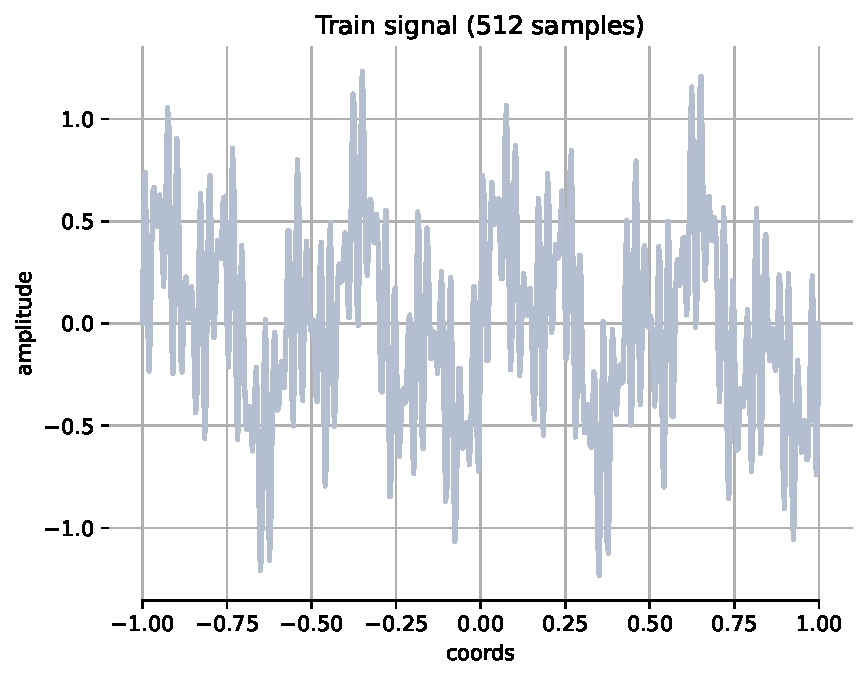
\includegraphics[width=\textwidth]{img/ch3/train_tones512.pdf}
        \caption{Input signal}
        \label{fig:gt-4freqs}
    \end{subfigure}
    \hfill
    \begin{subfigure}[b]{0.32\textwidth}
        \centering
        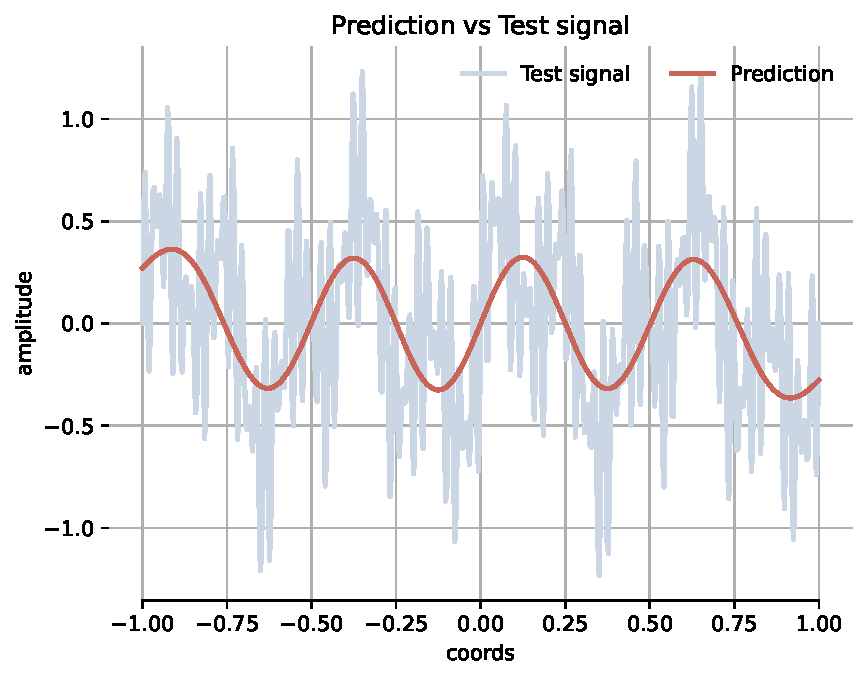
\includegraphics[width=\textwidth]{img/ch3/prediction_w10_smoothed.pdf}
        \caption{Reconstruction}
        \label{fig:rec-naive-w0}
    \end{subfigure}
    \hfill
    \begin{subfigure}[b]{0.32\textwidth}
        \centering
        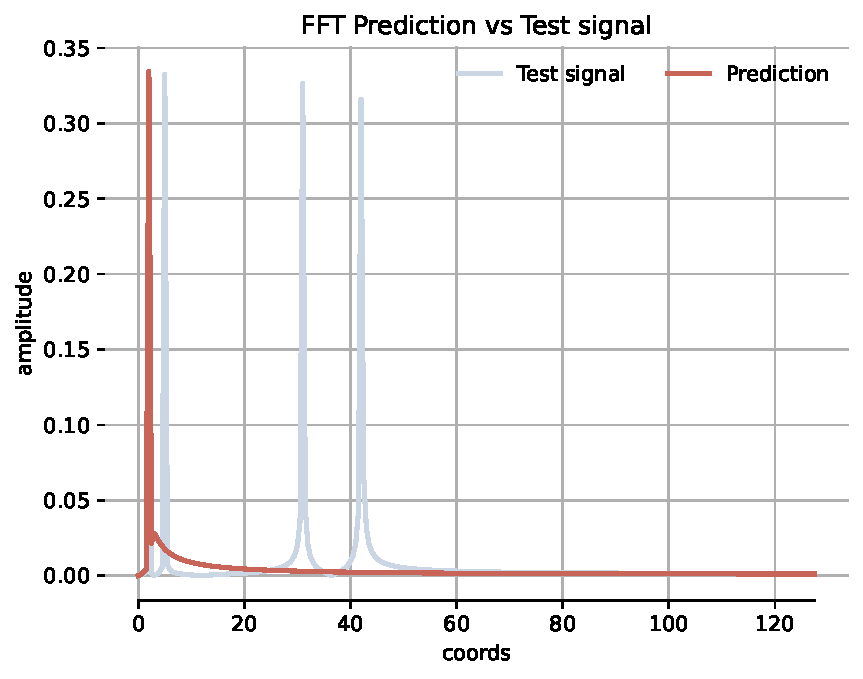
\includegraphics[width=\textwidth]{img/ch3/fft_w10_smoothed.pdf}
        \caption{Frequencies (FFT)}
        \label{fig:fft-smooth-4freqs}
    \end{subfigure}
    \label{f:4freqs-smoothed-reconstruction}
    \caption{Reconstruction of a signal with selected low and high frequencies using a network initialized with very low frequencies.}
\end{figure}


We believe this result is due to the network being initialized with frequencies lower than those present in the signal. Given that the sine function is periodic with a period of $2\pi$, we propose that the hyperparameter $\omega_0$ should always be multiplied by $2\pi$ to better establish a relationship between the initialization of the network's first layer and the range of frequencies represented by each atom in this layer.

Repeating the experiment with $\omega_0 = 10$ Hz, that is $10*2\pi$, we observe the expected behavior: the predicted wave in Figure \ref{fig:rec-2pi-w0} approximates the low-frequency portion of the signal. Notice how the FFT plot (Figure \ref{fig:fft-low-4freqs}) matches the peaks at 2 Hz and 5Hz, while the high frequency tones are not learned.

\begin{figure}[h!]
    \centering
    \begin{subfigure}[b]{0.38\textwidth}
        \centering
        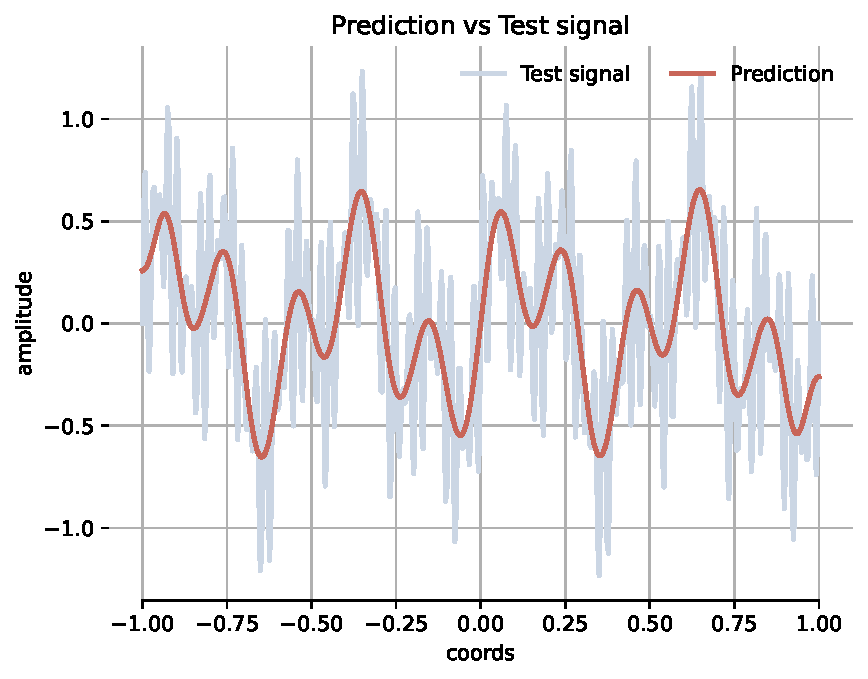
\includegraphics[width=\textwidth]{img/ch3/prediction_w0_2pi.pdf}
        \caption{Reconstruction}
        \label{fig:rec-2pi-w0}
    \end{subfigure}
    % \hfill
    \begin{subfigure}[b]{0.38\textwidth}
        \centering
        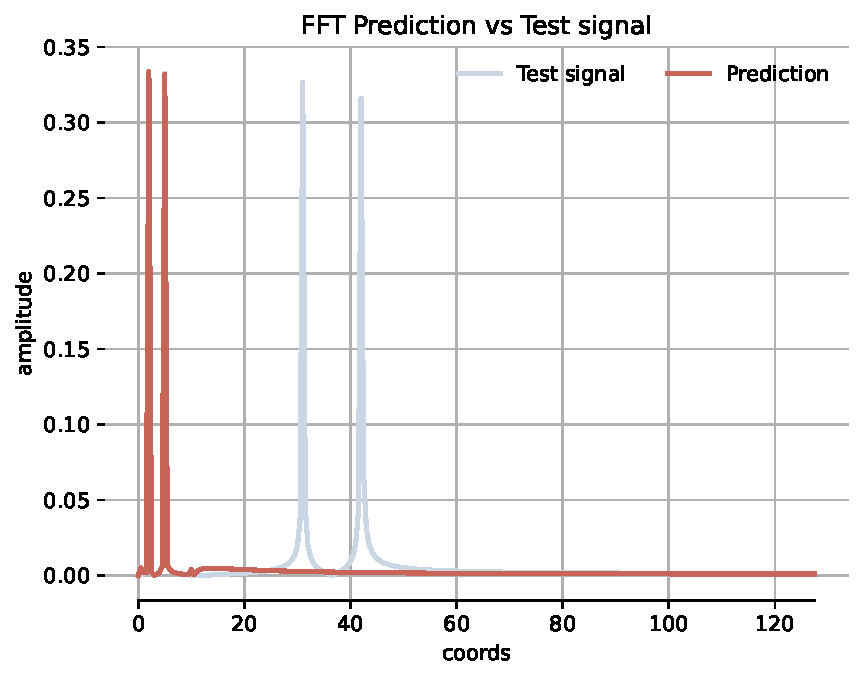
\includegraphics[width=\textwidth]{img/ch3/fft_w0_2pi.pdf}
        \caption{Frequencies (FFT)}
        \label{fig:fft-low-4freqs}
    \end{subfigure}
    \label{f:4freqs-low-reconstruction}
    \caption{Reconstruction of a signal with selected low and high frequencies, where the lower frequencies fall within the initialization range of the network's first layer.}
\end{figure}

Next we change the initialization of the network to frequencies between 25 and 45 Hz. As expected, that also succeeds in predicting the high-frequency tones but fails in capturing the low-frequency ones (Figures \ref{fig:rec-25-45} and \ref{fig:fft-25-45}). Moreover, by initializing the frequencies between 35 and 45 Hz, we are able to isolate the 42 Hz tone (Figures \ref{fig:rec-35-45} and \ref{fig:fft-35-45}).

\begin{figure}[h!]
    \centering
    \begin{subfigure}[b]{0.38\textwidth}
        \centering
        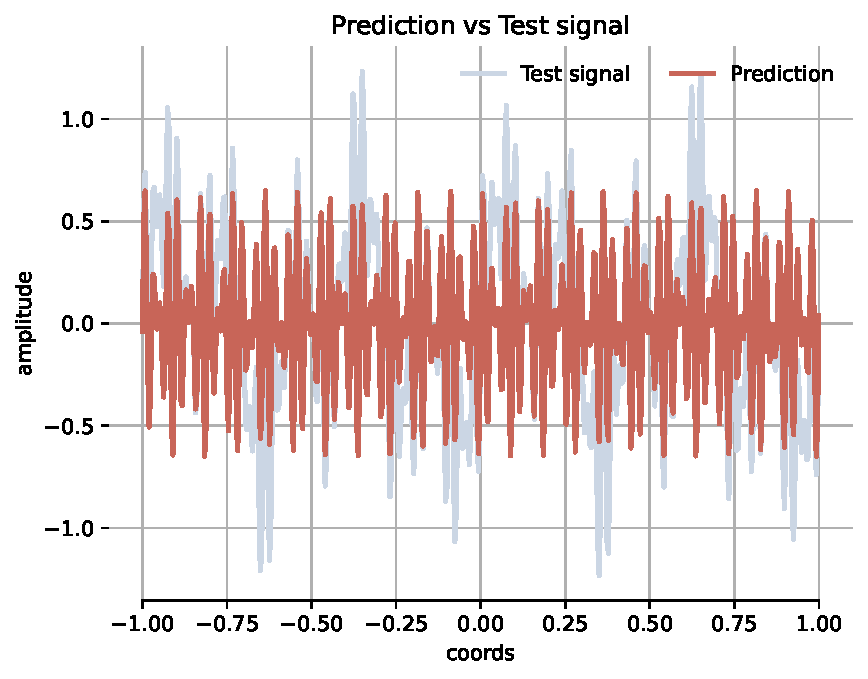
\includegraphics[width=\textwidth]{img/ch3/prediction_w25-45_2pi.pdf}
        \caption{$\omega_0 \in [25, 45]$Hz}
        \label{fig:rec-25-45}
    \end{subfigure}
    % \hfill
    \begin{subfigure}[b]{0.38\textwidth}
        \centering
        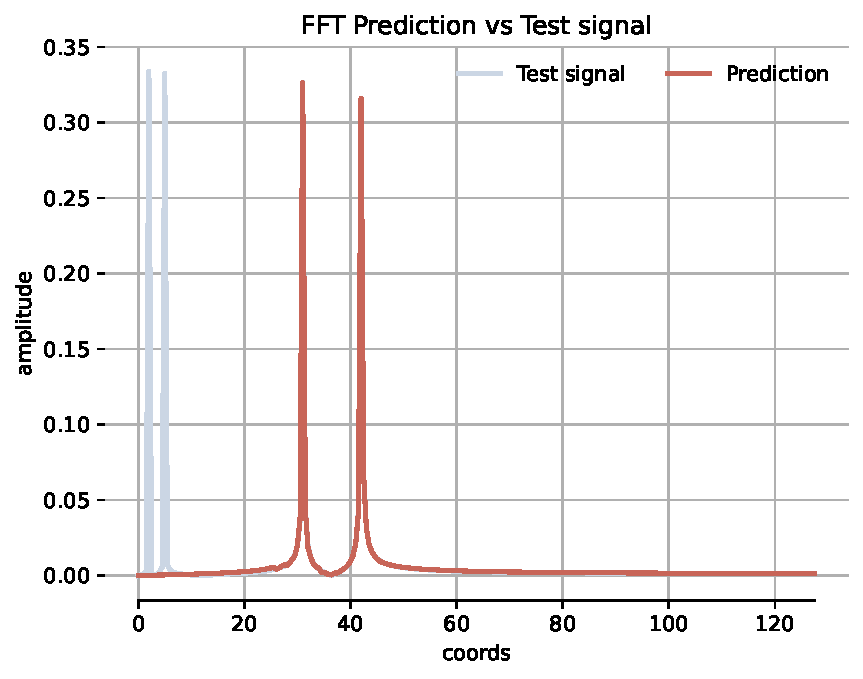
\includegraphics[width=\textwidth]{img/ch3/fft_w25-45.pdf}
        \caption{$\omega_0 \in [25, 45]$Hz}
        \label{fig:fft-25-45}
    \end{subfigure}
    \begin{subfigure}[b]{0.38\textwidth}
        \centering
        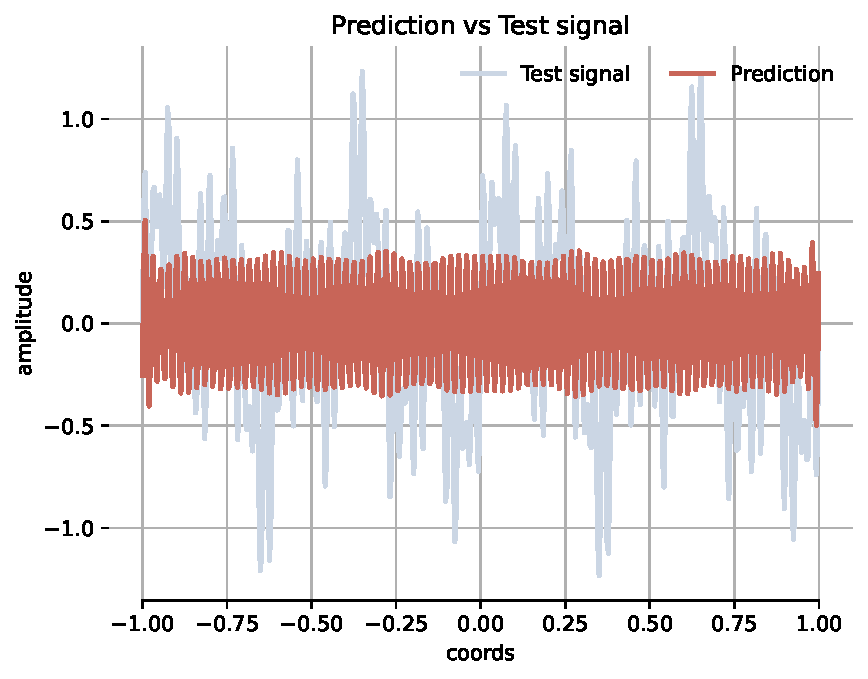
\includegraphics[width=\textwidth]{img/ch3/prediction_w35-45.pdf}
        \caption{$\omega_0 \in [35, 45]$Hz}
        \label{fig:rec-35-45}
    \end{subfigure}
    % \hfill
    \begin{subfigure}[b]{0.38\textwidth}
        \centering
        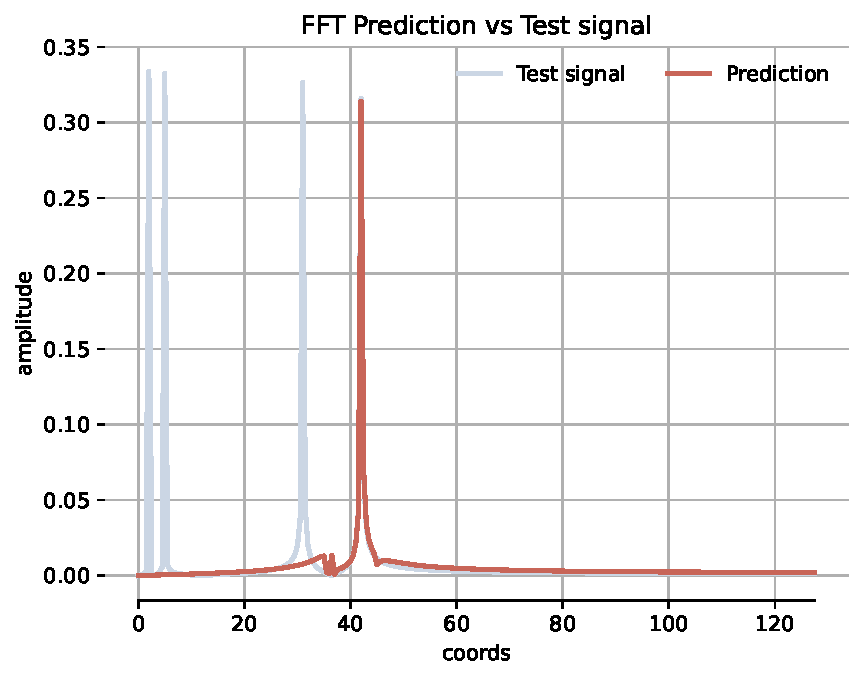
\includegraphics[width=\textwidth]{img/ch3/fft_w35-45.pdf}
        \caption{$\omega_0 \in [35, 45]$Hz}
        \label{fig:fft-35-45}
    \end{subfigure}
    \label{f:high-freqs-reconstruction}
    \caption{Reconstruction of the signal where only the higher frequencies fall within the initialization range of the network’s first layer.}
\end{figure}

Surprisingly, when we use a range of frequencies that encompasses all frequencies present in the input signal, for example $\omega_0 \in [-45, 45]$ Hz, the network does not perfectly fit the signal (Figure \ref{fig:rec-64-full-45}), and a mismatch between the frequencies of the network and of the input signal is evident in the Fast Fourier Transform plot (Figure \ref{fig:fft-64-full-45}). Our hypothesis is that this is due to the network's limited capacity, as it is a shallow network with only 64 neurons per layer. To test this, we repeated the experiment with larger models. Figures \ref{fig:rec-128-full-45} and \ref{fig:fft-128-full-45} show an improvement when the network width is increased to 128 neurons per layer. Note that with 256 neurons, the network can fit the signal perfectly, at least qualitatively, as the reconstructed signal appears to superimpose on the input signal both in the spatial (Figure \ref{fig:rec-256-full-45}) and the spectral (Figure \ref{fig:fft-256-full-45}) domains.

\begin{figure}[h!]
    \centering
    \begin{subfigure}[b]{0.32\textwidth}
        \centering
        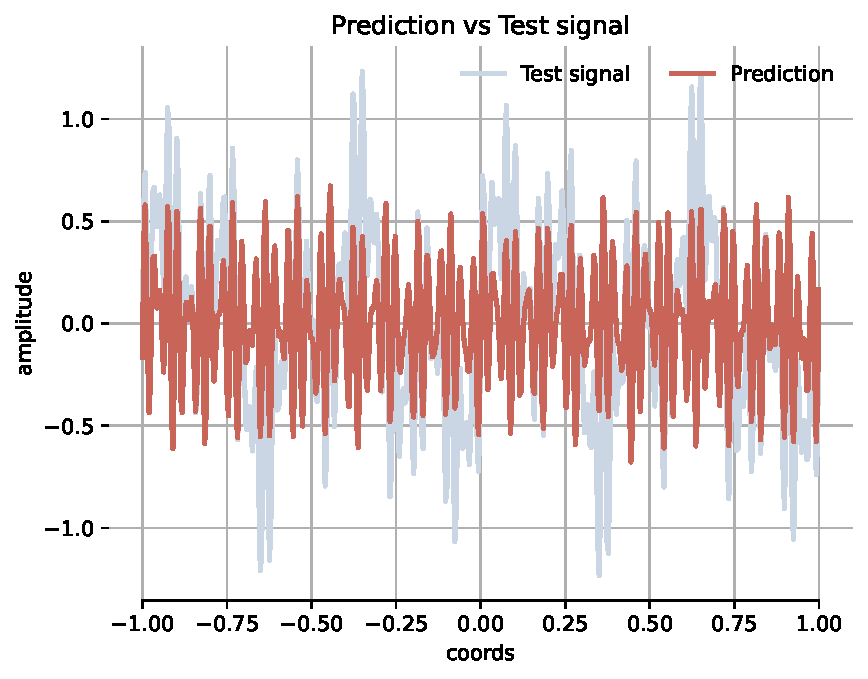
\includegraphics[width=\textwidth]{img/ch3/prediction_w45all_hf64.pdf}
        \caption{64 neurons}
        \label{fig:rec-64-full-45}
    \end{subfigure}
    \hfill
    \begin{subfigure}[b]{0.32\textwidth}
        \centering
        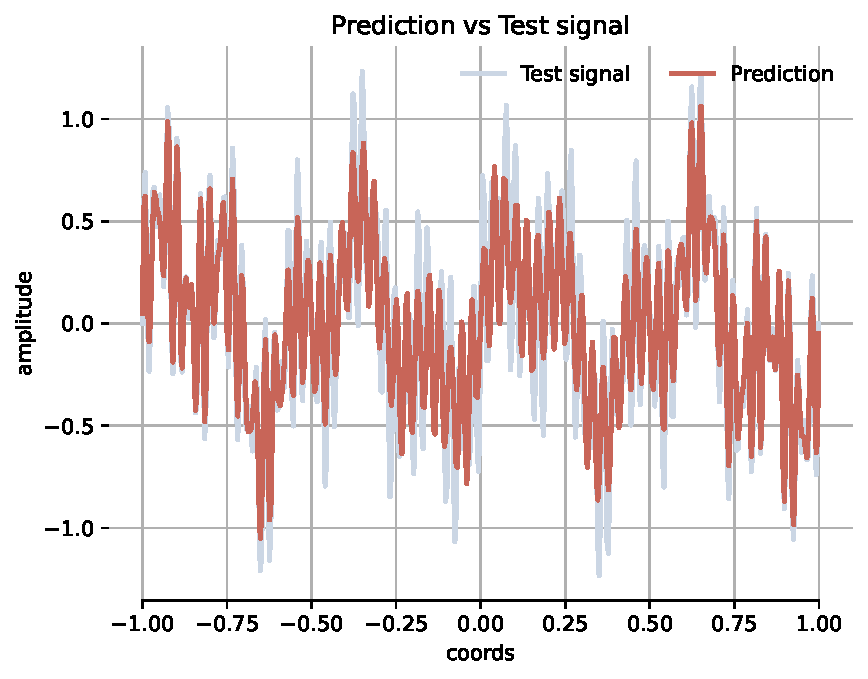
\includegraphics[width=\textwidth]{img/ch3/prediction_w45all_hf128.pdf}
        \caption{128 neurons}
        \label{fig:rec-128-full-45}
    \end{subfigure}
    \begin{subfigure}[b]{0.32\textwidth}
        \centering
        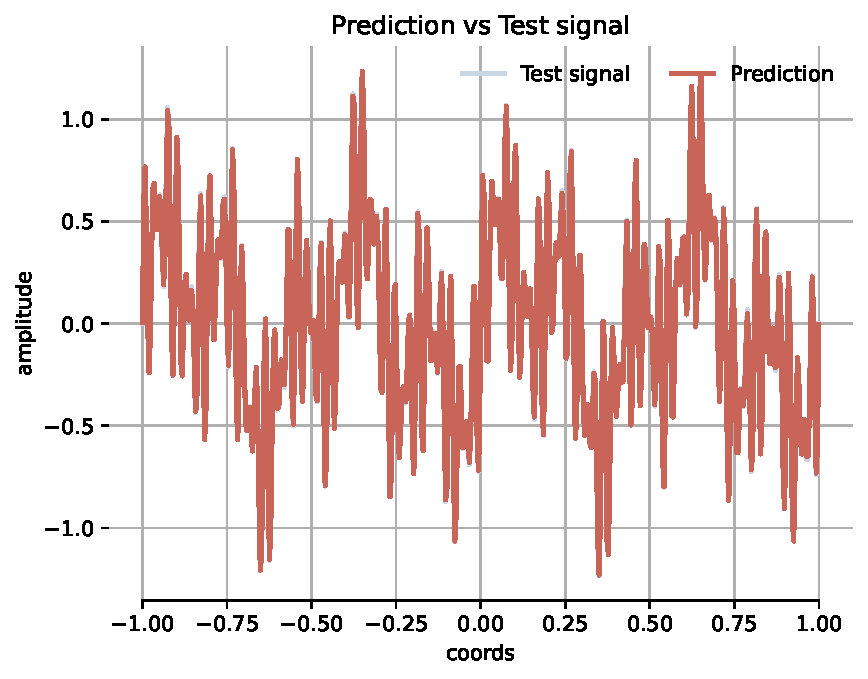
\includegraphics[width=\textwidth]{img/ch3/prediction_w45all_hf256.pdf}
        \caption{256 neurons}
        \label{fig:rec-256-full-45}
    \end{subfigure}
    \begin{subfigure}[b]{0.32\textwidth}
        \centering
        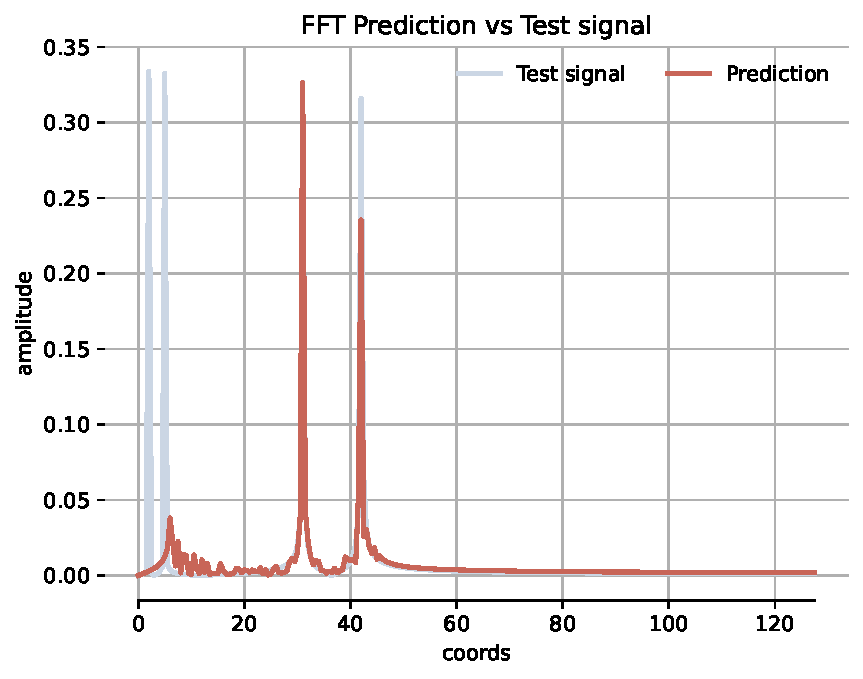
\includegraphics[width=\textwidth]{img/ch3/fft_w45all_hf64.pdf}
        \caption{64 neurons}
        \label{fig:fft-64-full-45}
    \end{subfigure}
    \hfill
    \begin{subfigure}[b]{0.32\textwidth}
        \centering
        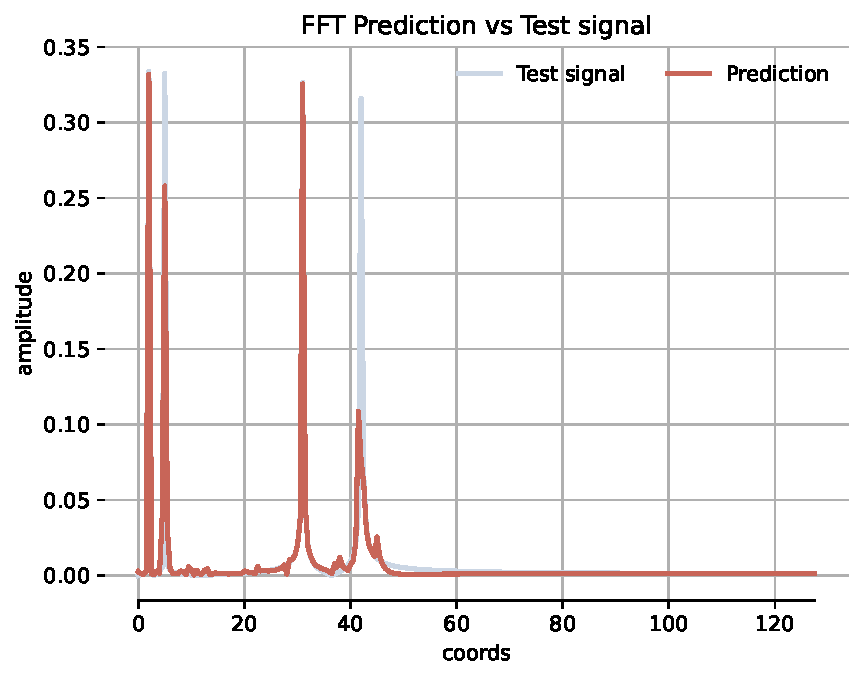
\includegraphics[width=\textwidth]{img/ch3/fft_w45all_hf128.pdf}
        \caption{128 neurons}
        \label{fig:fft-128-full-45}
    \end{subfigure}
    \begin{subfigure}[b]{0.32\textwidth}
        \centering
        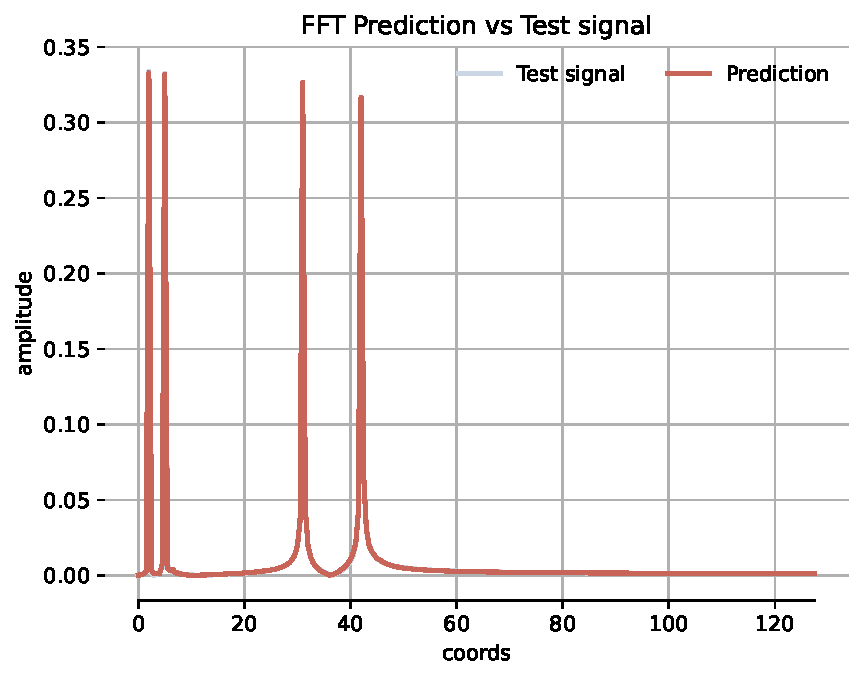
\includegraphics[width=\textwidth]{img/ch3/fft_w45all_hf256.pdf}
        \caption{256 neurons}
        \label{fig:fft-256-full-45}
    \end{subfigure}
    \label{fig:all-freqs-reconstruction}
    \caption{Reconstruction of the signal using networks with different width, all initialized with frequencies in $[-45, 45]$.}
\end{figure}


These experiments validate our hypothesis that a shallow network with only one layer of sinusoidal activation functions can filter a signal by band-limiting its frequency content, providing a spectral filter similar to those in MFN-based architectures. However, when we add a hidden sinusoidal layer to the network, it becomes much more challenging to isolate specific frequencies. Figure \ref{f:w10-1hl-64hf} shows the reconstruction of a sinusoidal network with one hidden layer and 64 neurons per layer, initialized with $\omega_0=10$ Hz. Similar to the experiment with a shallow network of 256 neurons, which was initialized with a broader spectrum of frequencies, the reconstruction seems to perfectly fit the input signal in both the spatial and spectral domains. Figures \ref{fig:4x-freqs-1hl-64hf} and \ref{fig:8x-freqs-1hl-64hf} present two zoomed-in views for a more detailed analysis. In this visualization, the network is evaluated in a grid with 512 samples within a much smaller interval, so most samples were not part of the training data. Notice that the reconstruction is smooth, presenting no spurious noise between the supervised samples.


\begin{figure}[h]
    \centering
    \begin{subfigure}[b]{0.4\textwidth}
        \centering
        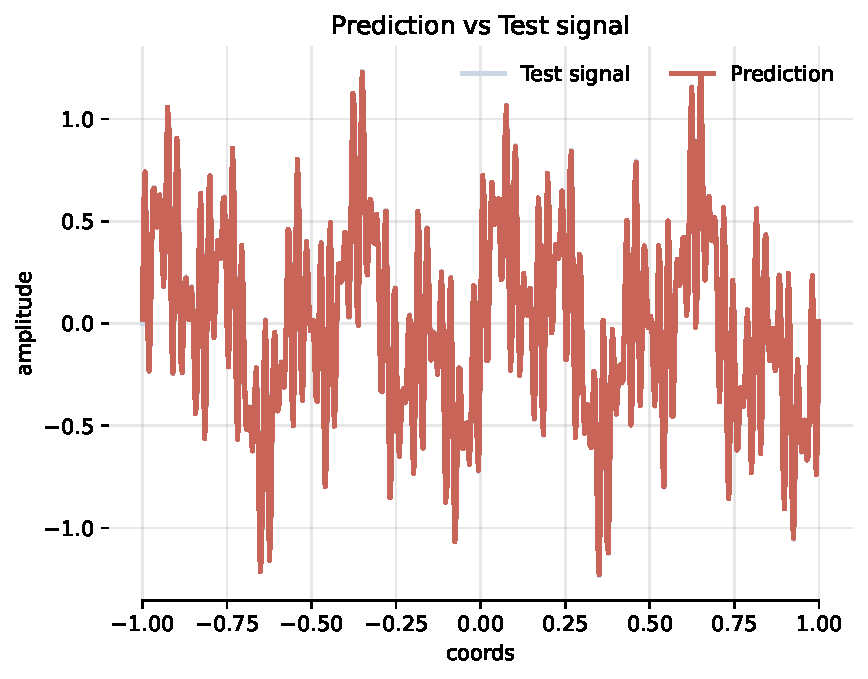
\includegraphics[width=\textwidth]{img/ch3/prediction_1hl_64hf_w10.pdf}
        \caption{Reconstruction}
        \label{fig:rec-freqs-1hl}
    \end{subfigure}
    % \hfill
    \begin{subfigure}[b]{0.4\textwidth}
        \centering
        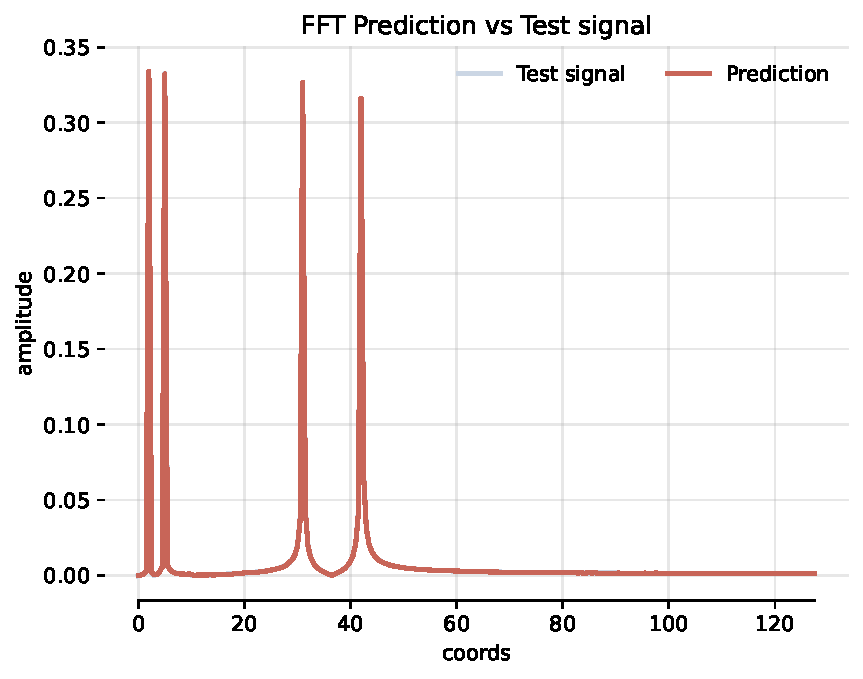
\includegraphics[width=\textwidth]{img/ch3/fft_1hl_64hf_w10.pdf}
        \caption{Frequencies}
        \label{fig:fft-freqs-1hl}
    \end{subfigure}
    
    \begin{subfigure}[b]{0.4\textwidth}
        \centering
        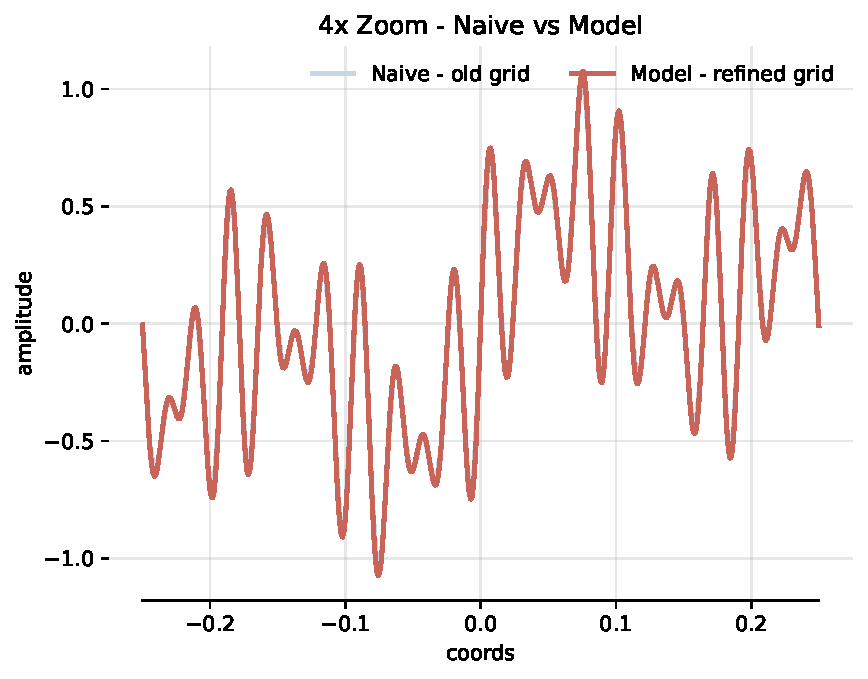
\includegraphics[width=\textwidth]{img/ch3/4x_zoom_1hl_64hf_w10.pdf}
        \caption{Zoom 4x}
        \label{fig:4x-freqs-1hl-64hf}
    \end{subfigure}
    % \hfill
    \begin{subfigure}[b]{0.4\textwidth}
        \centering
        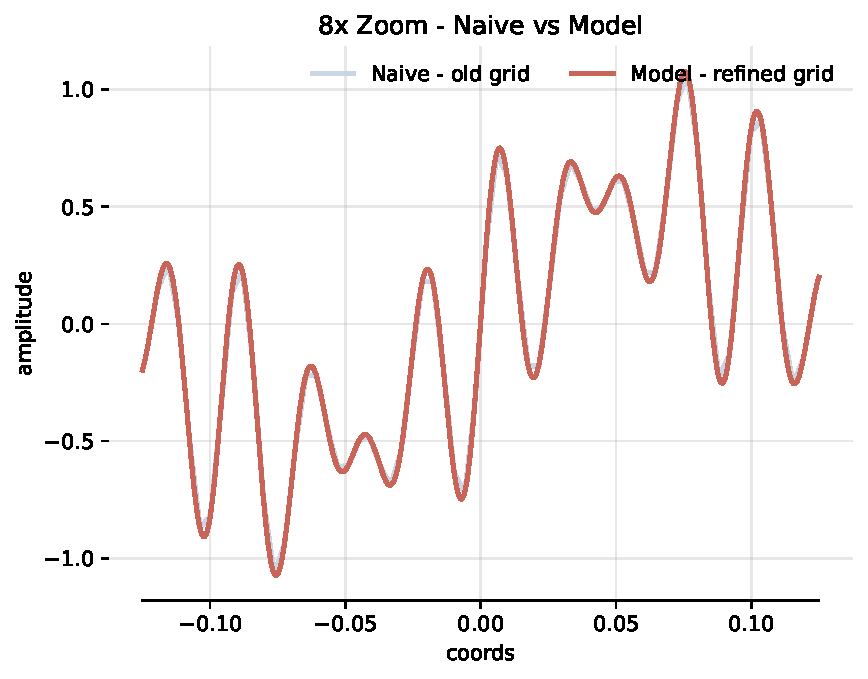
\includegraphics[width=\textwidth]{img/ch3/8x_zoom_1hl_64hf_w10.pdf}
        \caption{Zoom 8x}
        \label{fig:8x-freqs-1hl-64hf}
    \end{subfigure}
    \caption{Reconstruction using 1 hidden layer and 64 neurons per layer.}
    \label{f:w10-1hl-64hf}
\end{figure}

Although the width of the network was kept constant at 64 neurons, adding a single hidden layer significantly increases the size of the model, and thus its capacity, which could explain why it fits the signal better, even though it was initialized with lower frequencies. For instance, a shallow model with 64 neurons per layer has $192$ parameters, while a model with 1 hidden layer and 64 neurons per layer has $4352$ parameters.

To better understand the impact of the hidden layer, we conducted additional experiments, reducing the width of the networks with 1 hidden layer and increasing the width of those without hidden layers. For these experiments, all models were initialized with frequencies in the range $[-10*2\pi, 10*2\pi]$. Figure \ref{fig:rec-1hl-16hf-w10} shows the reconstruction of a model with 1 hidden layer and 16 neurons per layer, with a total of $320$ parameters. Note that this model still captures the high frequencies in the signal, although some noise is visible in its FFT (Figure \ref{fig:fft-1hl-16hf-w10}). However, the model with no hidden layers and 1024 neurons per layer is unable to capture any of the high frequencies (Figures \ref{fig:rec-0hl-1024-w10hf} and \ref{fig:fft-0hl-1024-w10hf}), despite having $3072$ parameters. We conclude that the hidden layer, rather than model size, is primarily responsible for this behavior.

\begin{figure}[h!]
    \centering
    \begin{subfigure}[b]{0.40\textwidth}
        \centering
        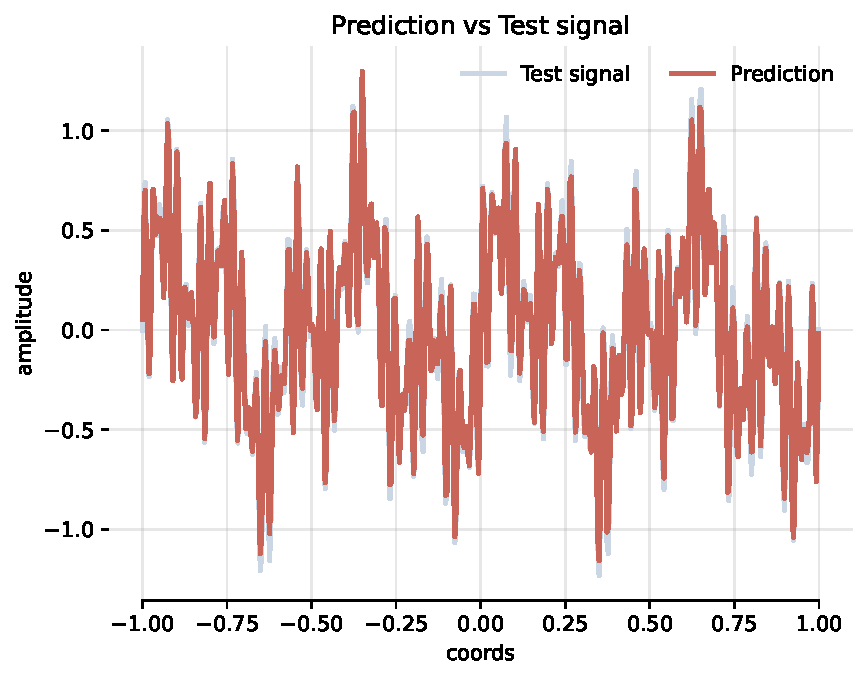
\includegraphics[width=\textwidth]{img/ch3/prediction_1hl_16hf_w10.pdf}
        \caption{1 hidden layer, 16 neurons}
        \label{fig:rec-1hl-16hf-w10}
    \end{subfigure}
    % \hfill
    \begin{subfigure}[b]{0.40\textwidth}
        \centering
        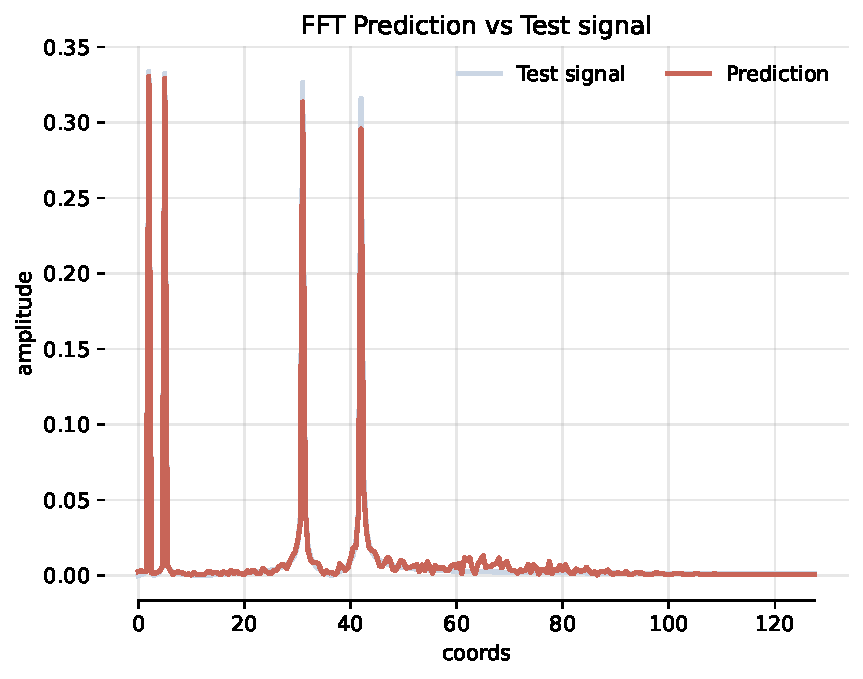
\includegraphics[width=\textwidth]{img/ch3/fft_1hl_16hf_w10.pdf}
        \caption{1 hidden layer, 16 neurons}
        \label{fig:fft-1hl-16hf-w10}
    \end{subfigure}
    
    \begin{subfigure}[b]{0.40\textwidth}
        \centering
        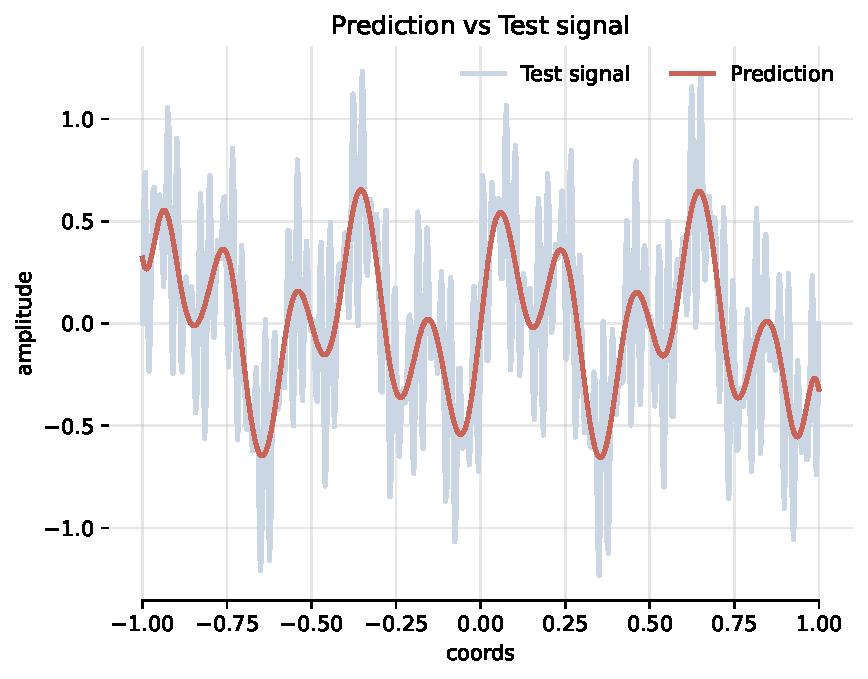
\includegraphics[width=\textwidth]{img/ch3/prediction_0hl_1024hf_w10.pdf}
        \caption{No hidden layers}
        \label{fig:rec-0hl-1024-w10hf}
    \end{subfigure}
    % \hfill
    \begin{subfigure}[b]{0.40\textwidth}
        \centering
        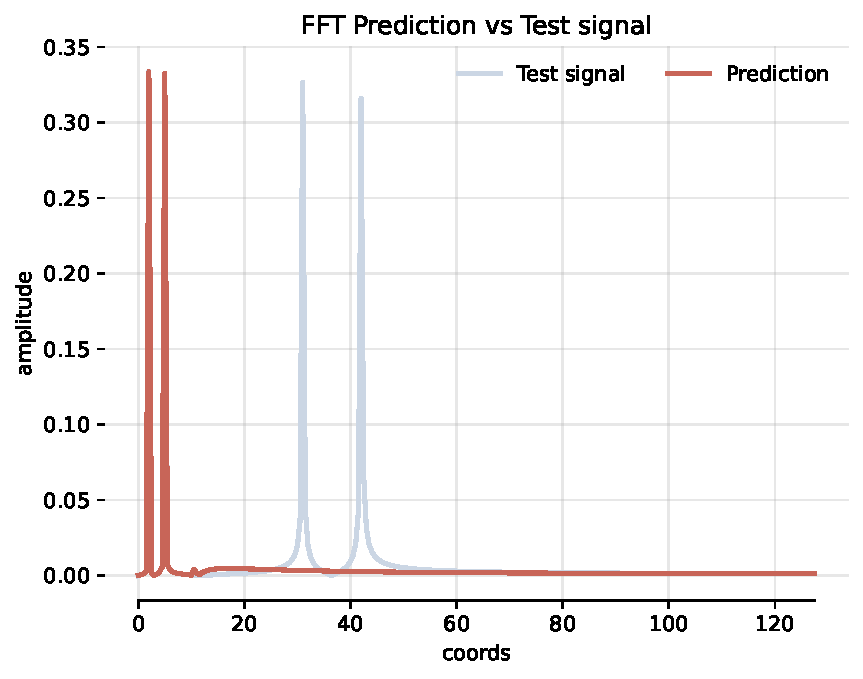
\includegraphics[width=\textwidth]{img/ch3/fft_0hl_1024hf_w10.pdf}
        \caption{No hidden layers}
        \label{fig:fft-0hl-1024-w10hf}
    \end{subfigure}
    \caption{Comparison of a smaller model with a single hidden layer to a larger model without hidden layers.}
    \label{f:hidden-layer-vs-no-hiddel-layer}
\end{figure}

We ran new experiments with networks initialized with frequencies in the range $[-35*2\pi, -25*2\pi] \cup [25*2\pi, 35*2\pi]$ and observed a similar phenomenon in the highest frequencies. Figure \ref{fig:rec-1hl-16hf-35w45} shows that a network with 1 hidden layer and 16 neurons per layer can capture the lower frequencies, despite showing some noise in its spectrum (Figure \ref{fig:fft-1hl-16hf-35w45}), while a network with no hidden layers and 1024 neurons per layer fails to capture the lower frequencies (Figures \ref{fig:rec-1hl-1024hf-35w45} and \ref{fig:fft-1hl-1024hf-35w45}).

\begin{figure}
    \centering
    \begin{subfigure}[b]{0.40\textwidth}
        \centering
        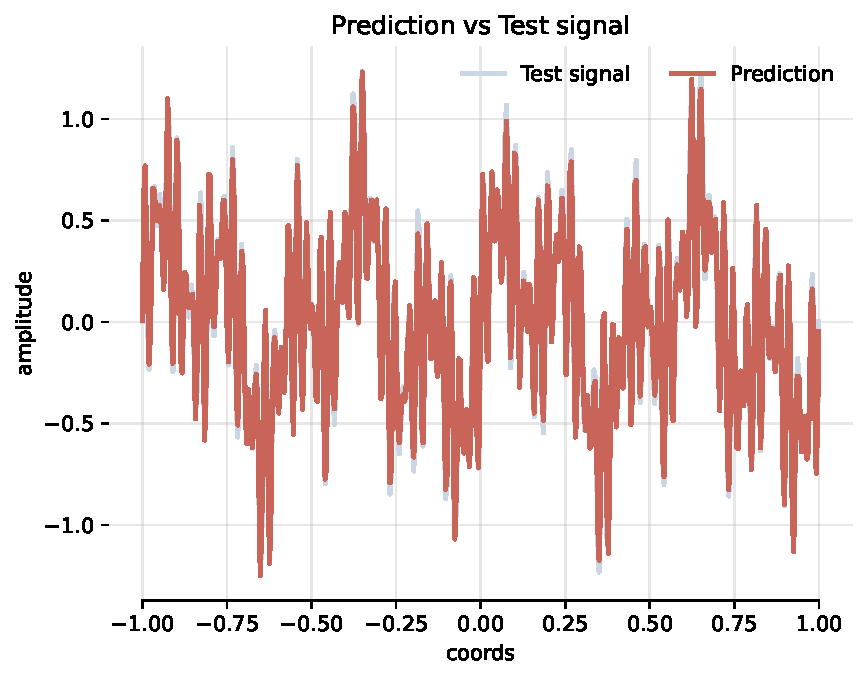
\includegraphics[width=\textwidth]{img/ch3/prediction_1hl_16hf_35w45.pdf}
        \caption{1 hidden layer, 16 neurons}
        \label{fig:rec-1hl-16hf-35w45}
    \end{subfigure}
    % \hfill
    \begin{subfigure}[b]{0.40\textwidth}
        \centering
        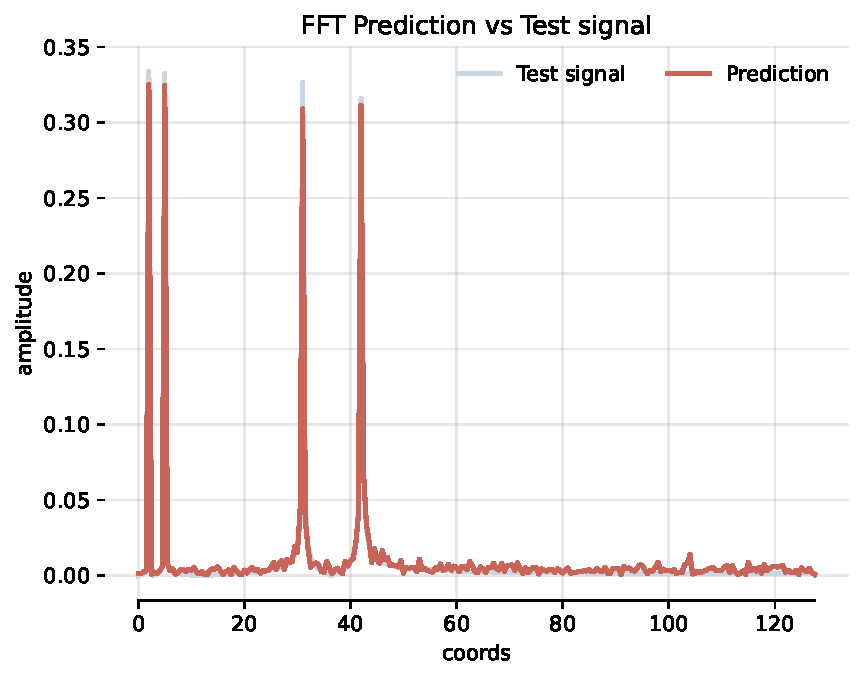
\includegraphics[width=\textwidth]{img/ch3/fft_1hl_16hf_35w45.pdf}
        \caption{1 hidden layer, 16 neurons}
        \label{fig:fft-1hl-16hf-35w45}
    \end{subfigure}
    
    \begin{subfigure}[b]{0.40\textwidth}
        \centering
        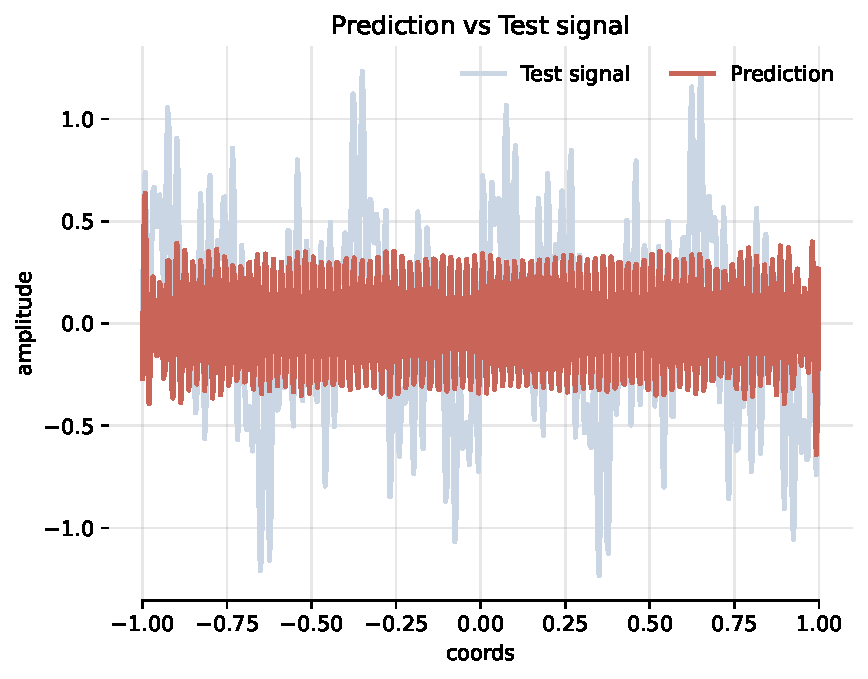
\includegraphics[width=\textwidth]{img/ch3/prediction_1hl_1024hf_35w45.pdf}
        \caption{No hidden layers}
        \label{fig:rec-1hl-1024hf-35w45}
    \end{subfigure}
    % \hfill
    \begin{subfigure}[b]{0.40\textwidth}
        \centering
        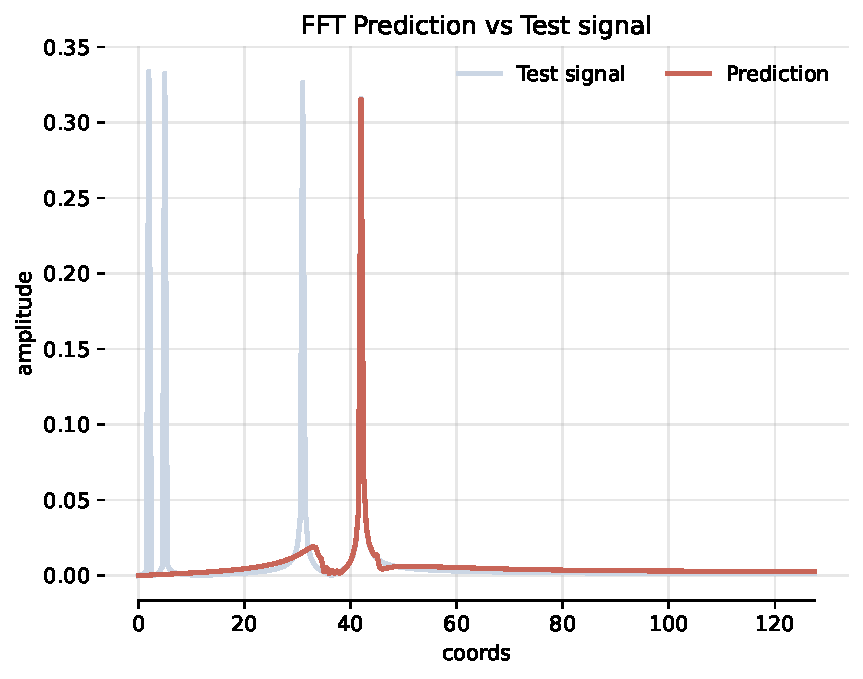
\includegraphics[width=\textwidth]{img/ch3/fft_1hl_1024hf_35w45.pdf}
        \caption{No hidden layers}
        \label{fig:fft-1hl-1024hf-35w45}
    \end{subfigure}
    \caption{Comparison between smaller model with 1 hidden layer and bigger model without hidden layer when models are initialized only with high frequencies.}
    \label{f:hiddenlayer-vs-nohl-high-frequencies}
\end{figure}


We conclude that a sinusoidal neural network with no hidden layers can effectivelly filter and decompose the frequencies of a sinal. However, in general, it not straightforward to decompose the frequencies of a signal using a sinusoidal deep network with at least one hidden layer.

\pagebreak

\subsection{Learning and filtering stochastic signals}

%     - Diverging by using high frequencies. Show how the network diverges when initialized with very high frequencies.


After experimenting with signals containing a few controlled frequencies, we procedurally generated stochastic signals using a technique known as Perlin Noise (\cite{perlin-1985}). This approach allows us to analyze how a sinusoidal model learns a distribution of frequencies across a broad range. For the following experiments, we sampled 2048 points uniformly from the interval $[-1, 1]$, yielding a sampling rate of 1/1024. According to the Shannon-Nyquist sampling theorem, this limits us to frequencies up to 512 Hz. The parameters for generating the Perlin Noise signal were: scale = 10; octaves = 16; persistence = 1.4.

We began by training a shallow sinusoidal network as a sanity check. The expectation was for the network to capture only the lowest frequencies, up to the range determined by its initialization parameter, $\omega_0$. We used a network with 512 hidden neurons per layer, varying the value of $\omega_0$. Figure \ref{f:rec-noise-shallow} shows the reconstruction in both spatial and frequency domains for $\omega_0 \in \{8, 64, 128\}$ Hz. Note that the FFT plot displays a distribution of frequencies up to 512 Hz, with higher amplitudes for the lower frequencies. As expected, the results resemble smoothed versions of the signal, as the network captures only the frequencies up to the value of $\omega_0$.

\begin{figure}[h]
    \centering
    \begin{subfigure}[b]{0.32\textwidth}
        \centering
        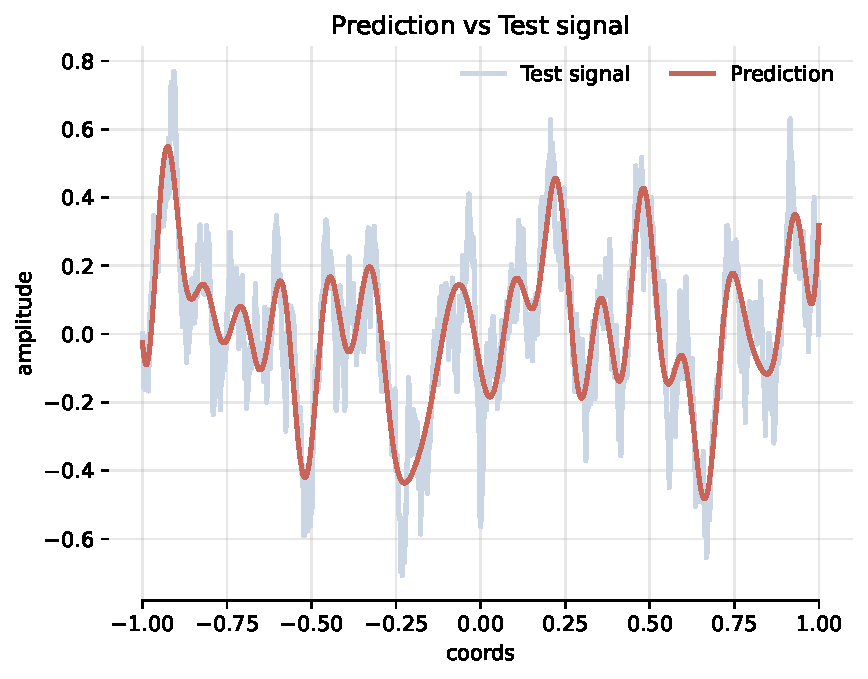
\includegraphics[width=\textwidth]{img/ch3/pred-noise-h0-w8.pdf}
        \caption{$\omega_0=8$}
        \label{fig:rec-noise-shallow-w8}
    \end{subfigure}
    \hfill
    \begin{subfigure}[b]{0.32\textwidth}
        \centering
        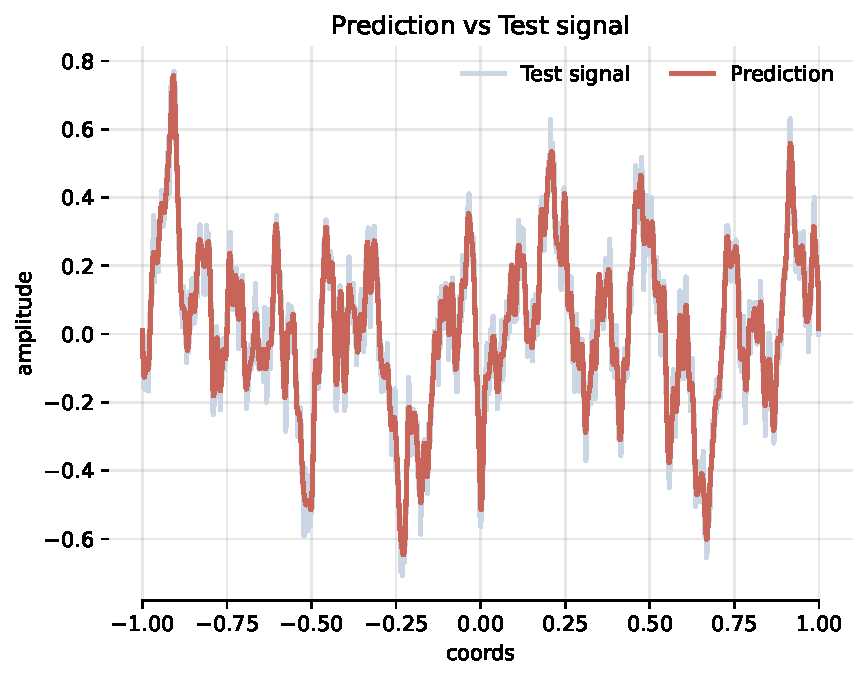
\includegraphics[width=\textwidth]{img/ch3/pred-noise-h0-w64.pdf}
        \caption{$\omega_0=64$}
        \label{fig:rec-noise-shallow-w64}
    \end{subfigure}
    \hfill
    \begin{subfigure}[b]{0.32\textwidth}
        \centering
        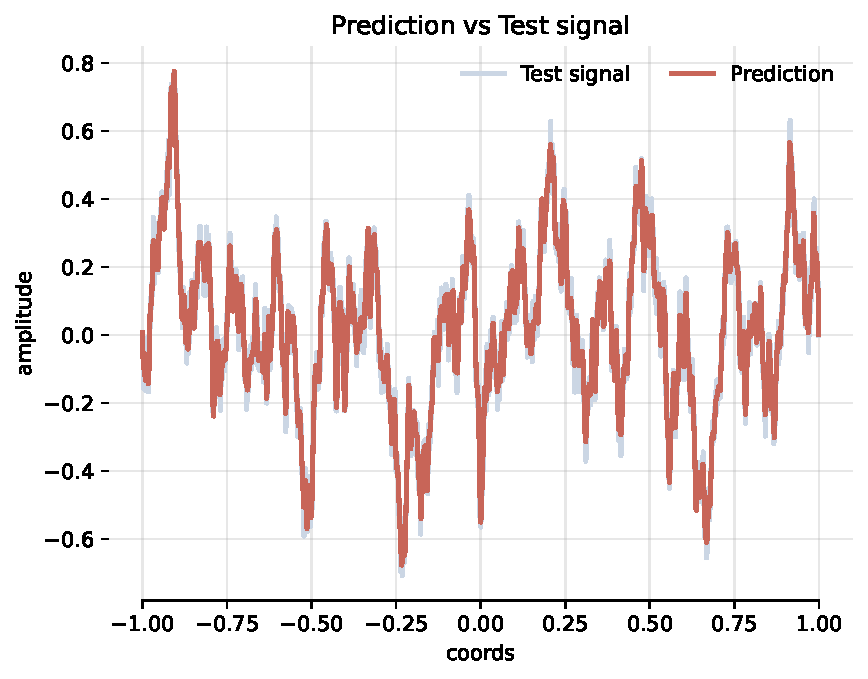
\includegraphics[width=\textwidth]{img/ch3/pred-noise-h0-w128.pdf}
        \caption{$\omega_0=128$}
        \label{fig:rec-noise-shallow-w128}
    \end{subfigure}

    \begin{subfigure}[b]{0.32\textwidth}
        \centering
        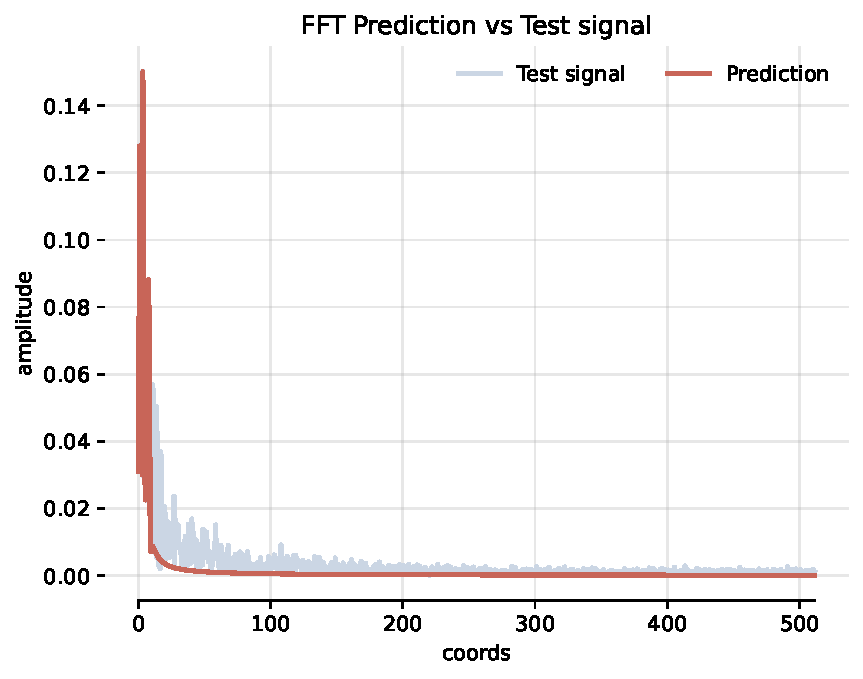
\includegraphics[width=\textwidth]{img/ch3/fft-noise-h0-w8.pdf}
        \caption{$\omega_0=8$}
        \label{fig:fft-noise-shallow-w8}
    \end{subfigure}
    \hfill
    \begin{subfigure}[b]{0.32\textwidth}
        \centering
        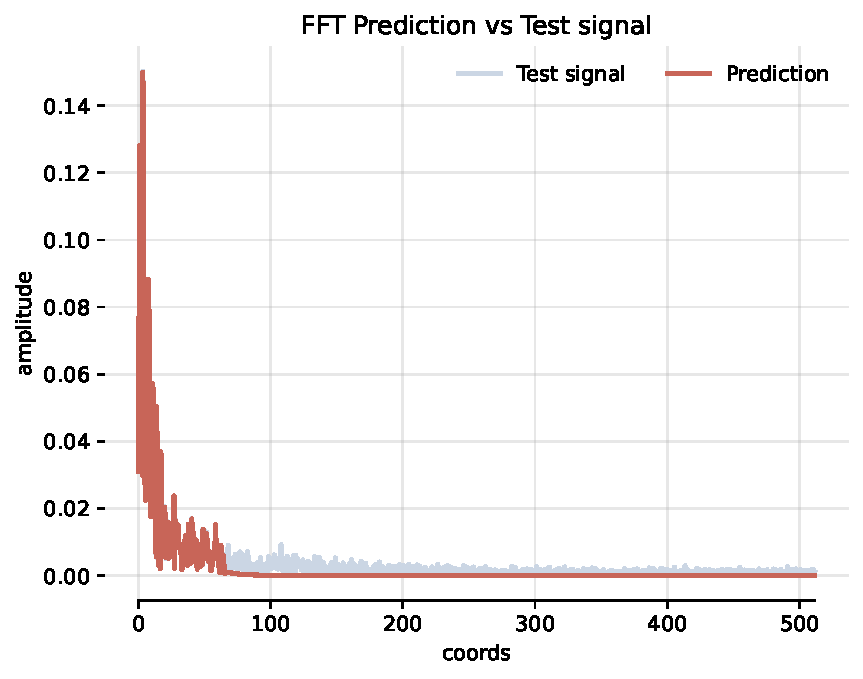
\includegraphics[width=\textwidth]{img/ch3/fft-noise-h0-w64.pdf}
        \caption{$\omega_0=64$}
        \label{fig:fft-noise-shallow-w64}
    \end{subfigure}
    \hfill
    \begin{subfigure}[b]{0.32\textwidth}
        \centering
        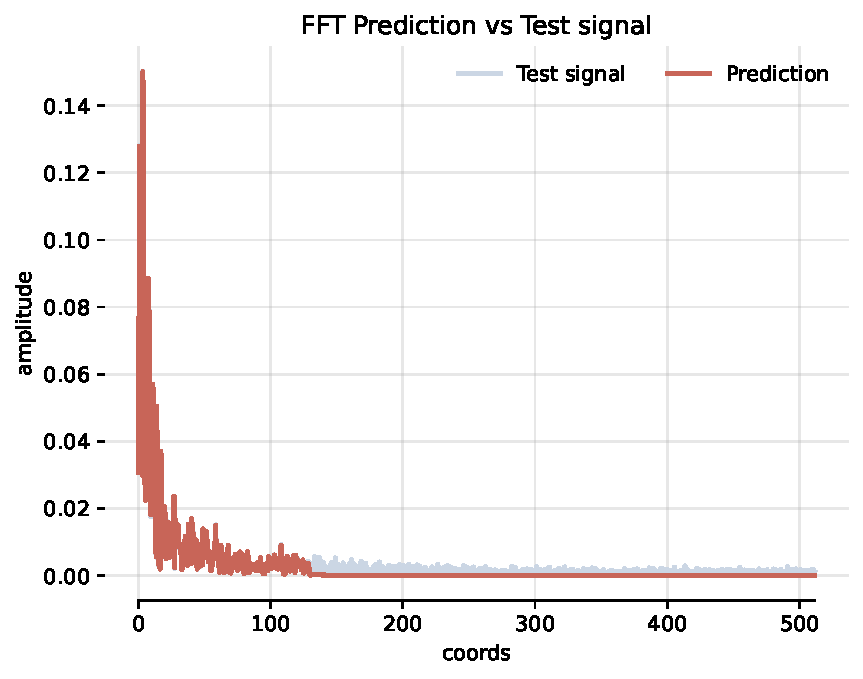
\includegraphics[width=\textwidth]{img/ch3/fft-noise-h0-w128.pdf}
        \caption{$\omega_0=128$}
        \label{fig:fft-noise-shallow-w128}
    \end{subfigure}
    \caption{Reconstruction of a stochastic signal using shallow sinusoidal networks initilized with differente frequency ranges.}
    \label{f:rec-noise-shallow}
\end{figure}

As we increase $\omega_0$ to capture higher frequencies, we observe a phenomenon similar to that seen in Figure \ref{fig:fft-64-full-45}: the model's performance deteriorates for some of the lower frequencies, and noise is introduced due to insufficient capacity. This situation is illustrated in Figure \ref{f:rec-noise-shallow-hf512-w256}.

\begin{figure}[h]
    \centering
    \begin{subfigure}[b]{0.40\textwidth}
        \centering
        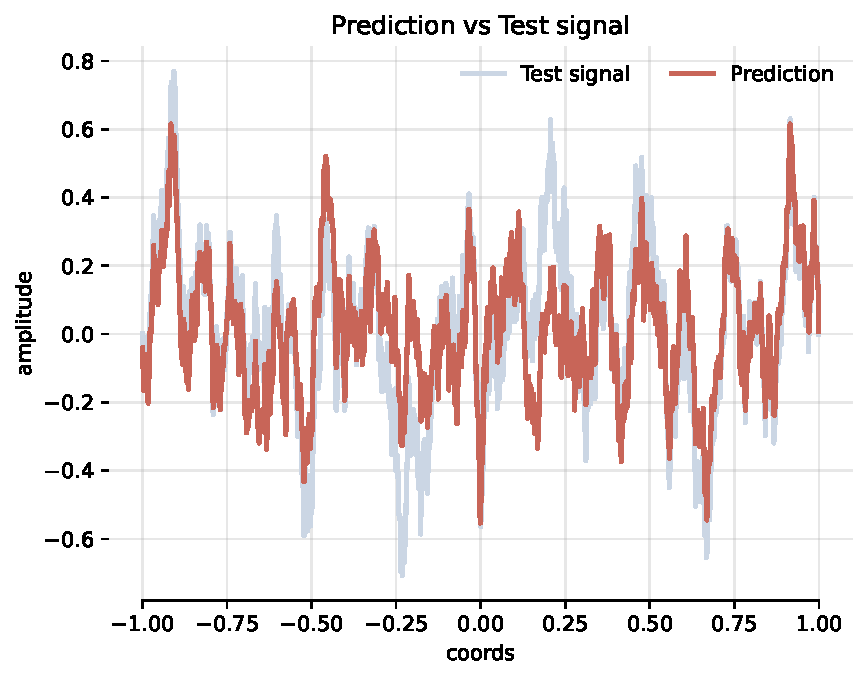
\includegraphics[width=\textwidth]{img/ch3/pred-noise-h0-hf512-w256.pdf}
        \caption{}
    \end{subfigure}
    % \hfill
    \begin{subfigure}[b]{0.40\textwidth}
        \centering
        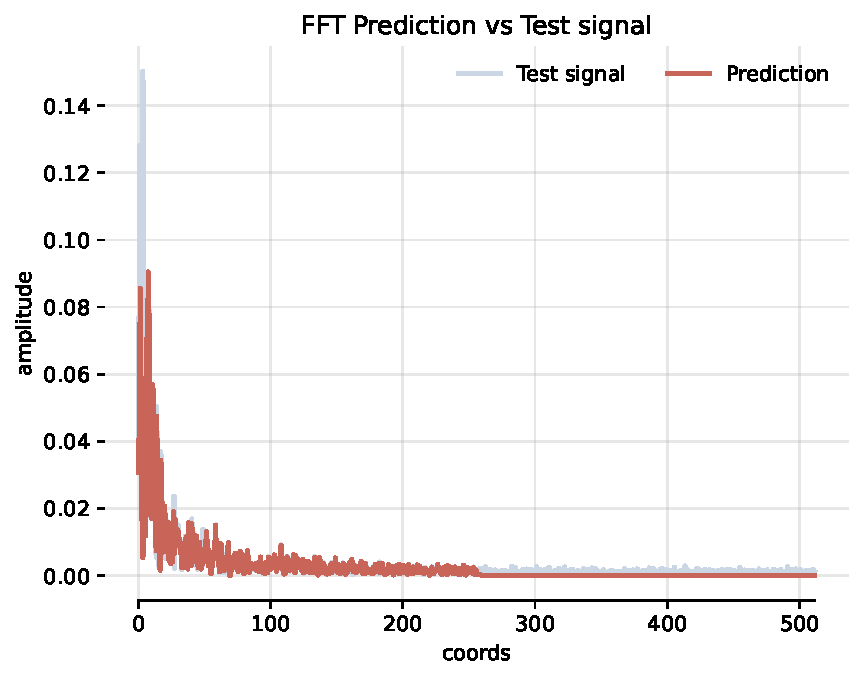
\includegraphics[width=\textwidth]{img/ch3/fft-noise-h0-hf512-w256.pdf}
        \caption{}
        % \label{fig:fft-noise-shallow-hf512-w256}
    \end{subfigure}
    \caption{Reconstruction of signal (A) and frequencies (B) using 512 neurons per layer and $\omega_0=256$}
    \label{f:rec-noise-shallow-hf512-w256}
\end{figure}

We also noticed significant oscillations in the loss function curve in experiments involving larger frequencies. Figure \ref{f:loss-noise-comparison-hl0-hf512} presents the mean squared error per epoch during the training of networks with $\omega_0=64$ and $\omega_0=256$. Based on these observations, we reduced the learning rate to 0.0001, increased the number of training epochs to 400, and ran new experiments. Figure \ref{f:full-noise-hf4096-w512} shows the results from these updated experiments, using 4096 neurons per layer, with zoomed-in views for detailed analysis.

\begin{figure}[h]
    \centering
    \begin{subfigure}[b]{0.45\textwidth}
        \centering
        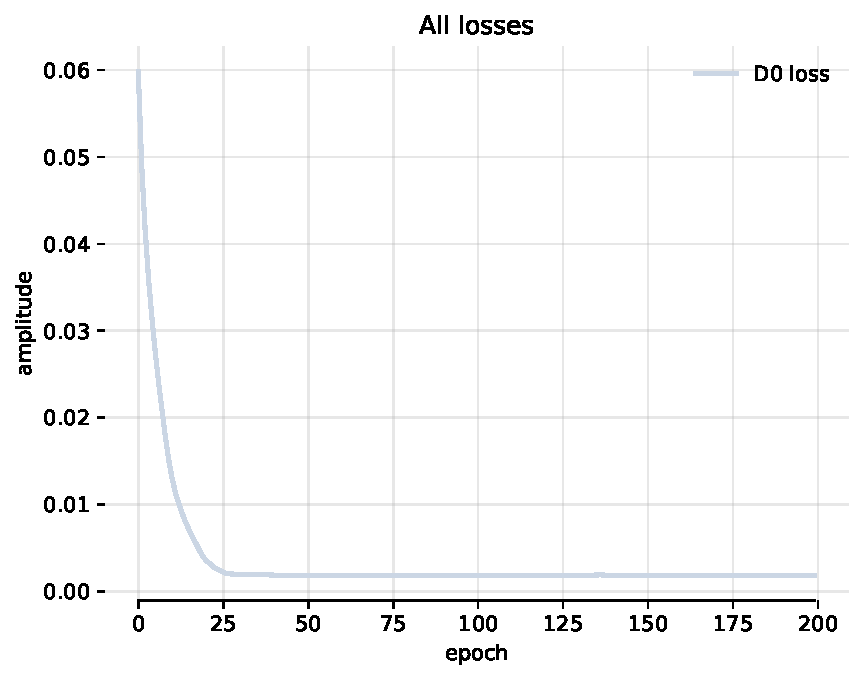
\includegraphics[width=\textwidth]{img/ch3/loss-noise-hl0-hf512-w64.pdf}
        \caption{$\omega_0=64$}
        \label{fig:loss-hf512-w64}
    \end{subfigure}
    \begin{subfigure}[b]{0.45\textwidth}
        \centering
        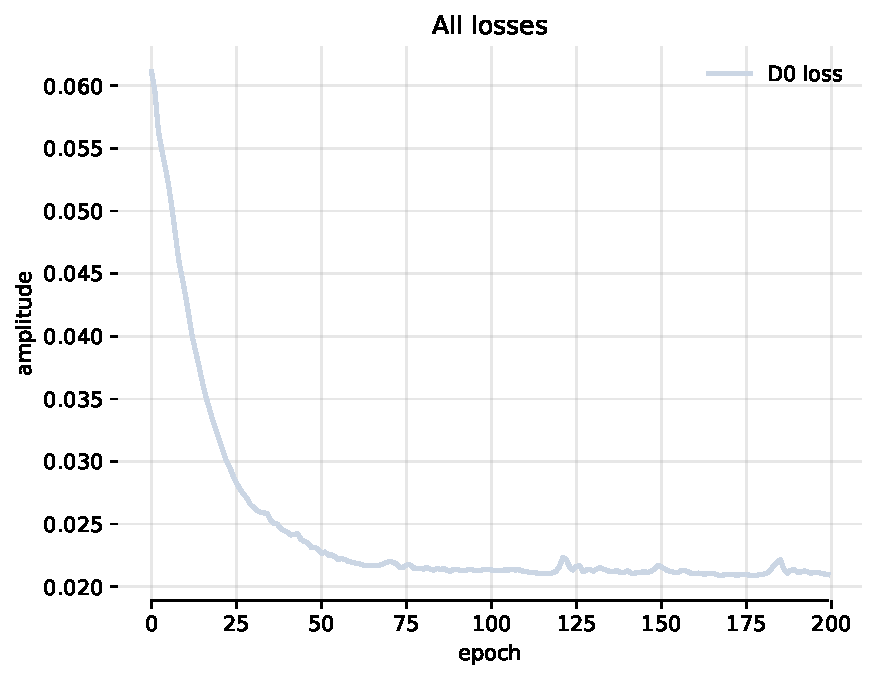
\includegraphics[width=\textwidth]{img/ch3/loss-noise-hl0-hf512-w256.pdf}
        \caption{$\omega_0=256$}
        \label{fig:loss-hf512-w256}
    \end{subfigure}
    \caption{Mean squared error per epoch.}
    \label{f:loss-noise-comparison-hl0-hf512}
\end{figure}


\begin{figure}[h]
    \centering
    \begin{subfigure}[b]{0.32\textwidth}
        \centering
        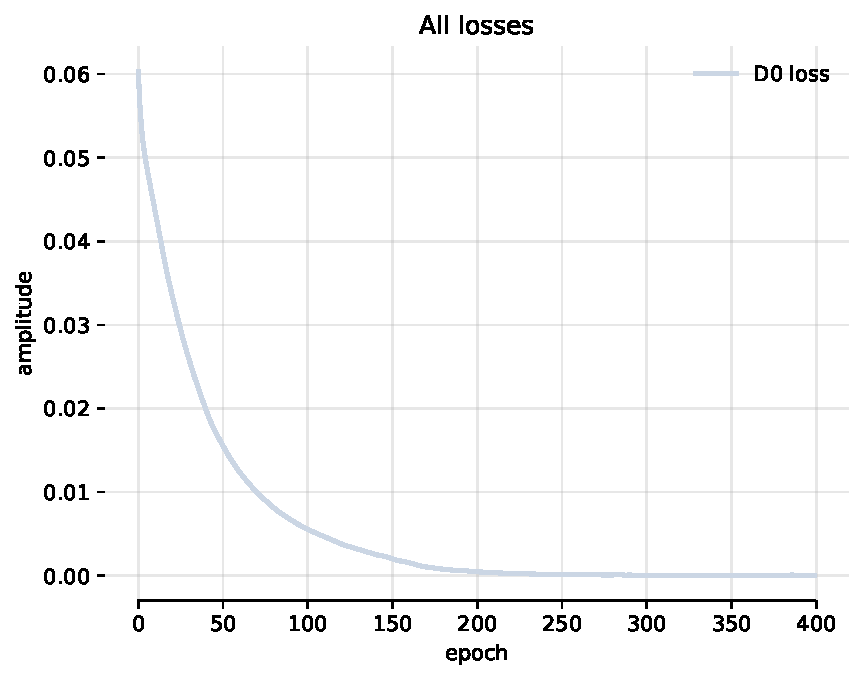
\includegraphics[width=\textwidth]{img/ch3/loss-noise-hf4096-w512.pdf}
        \caption{Loss}
    \end{subfigure}
    \begin{subfigure}[b]{0.32\textwidth}
        \centering
        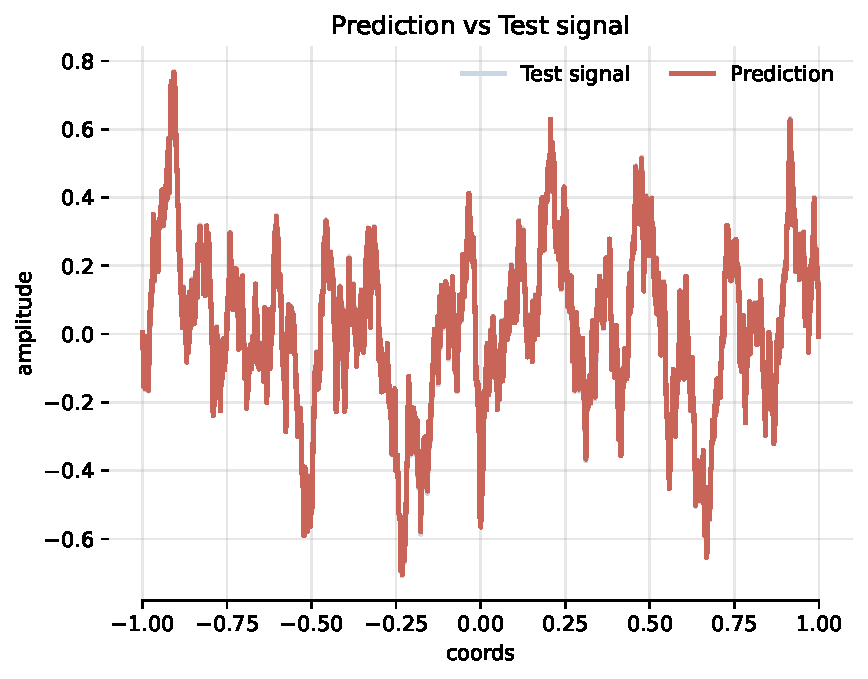
\includegraphics[width=\textwidth]{img/ch3/pred-noise-hf4096-w512.pdf}
        \caption{Reconstruction}
    \end{subfigure}
    \begin{subfigure}[b]{0.32\textwidth}
        \centering
        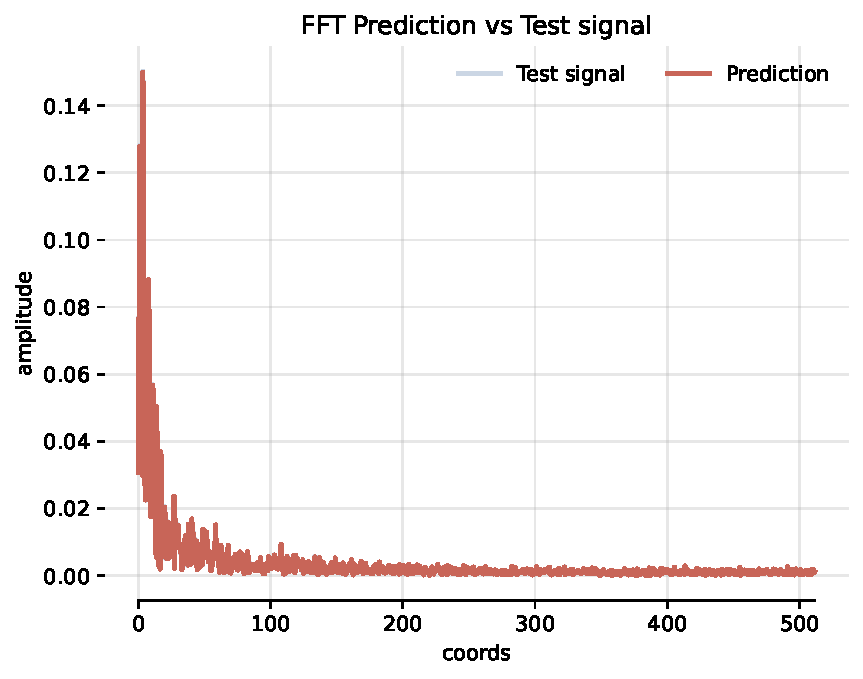
\includegraphics[width=\textwidth]{img/ch3/fft-noise-hf4096-w512.pdf}
        \caption{Frequencies}
    \end{subfigure}

    \begin{subfigure}[b]{0.32\textwidth}
        \centering
        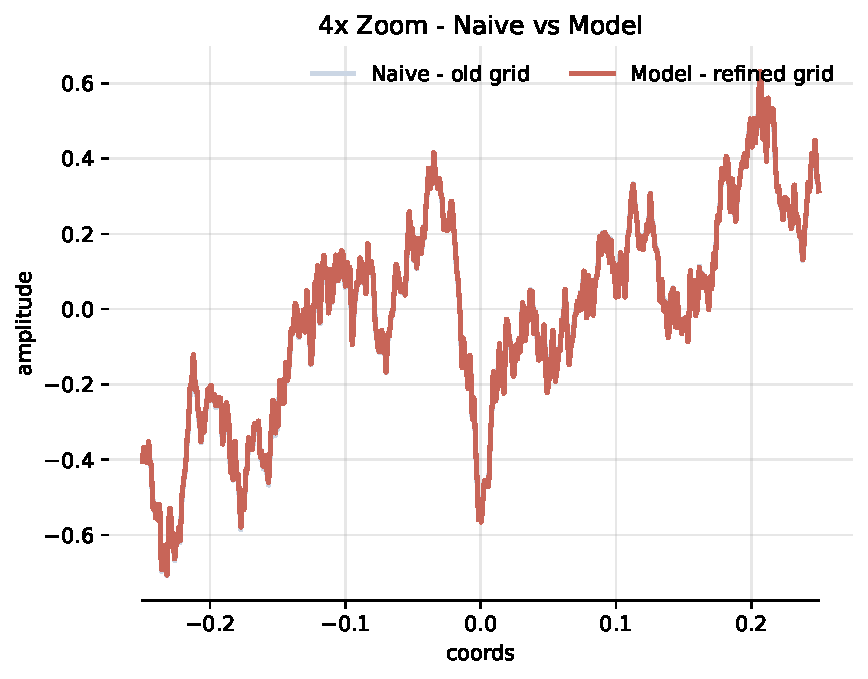
\includegraphics[width=\textwidth]{img/ch3/noise-4x-hf4096-w512.pdf}
        \caption{4x zoom}
    \end{subfigure}
    \begin{subfigure}[b]{0.32\textwidth}
        \centering
        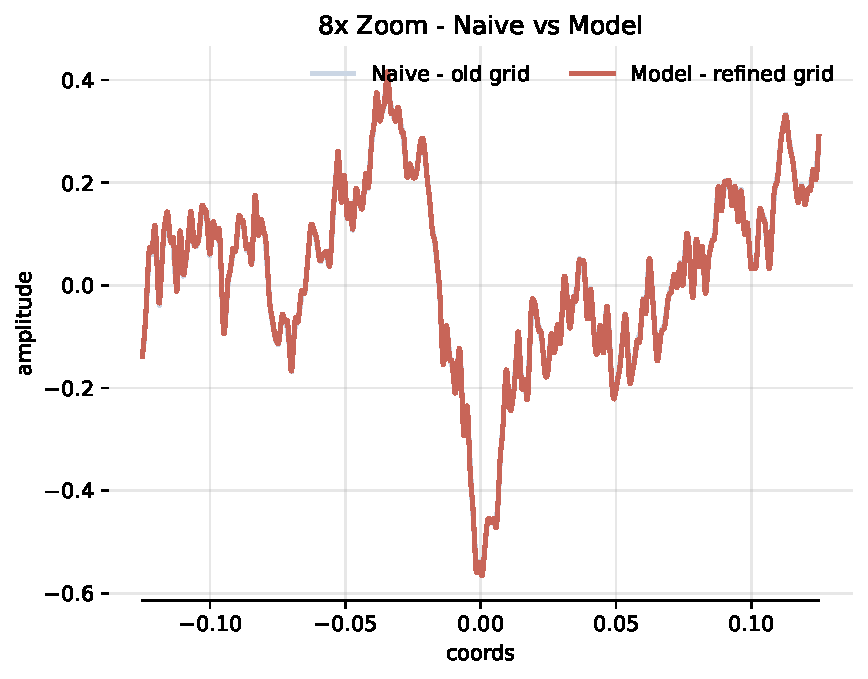
\includegraphics[width=\textwidth]{img/ch3/noise-8x-hf4096-w512.pdf}
        \caption{8x zoom}
    \end{subfigure}
    \begin{subfigure}[b]{0.32\textwidth}
        \centering
        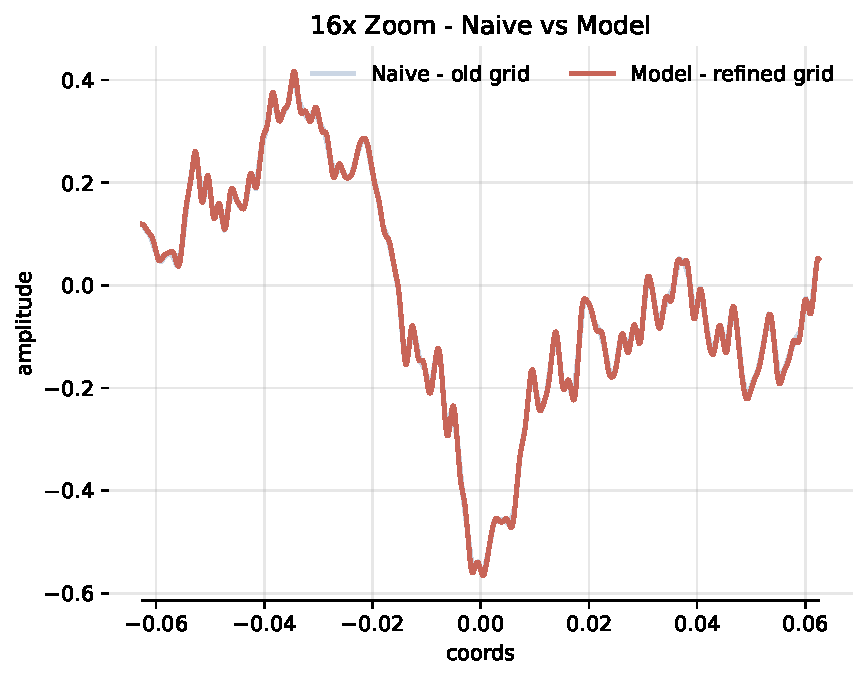
\includegraphics[width=\textwidth]{img/ch3/noise-16x-hf4096-w512.pdf}
        \caption{16x zoom}
    \end{subfigure}
    \caption{Reconstruction results using a shallow network with 4096 neurons per layer and $\omega_0=512$}
    \label{f:full-noise-hf4096-w512}
\end{figure}


In the following experiments, we employed sinusoidal neural networks with one hidden layer. The primary question we wanted to investigate was: \emph{can smaller, but deeper, networks learn bounded frequencies?} The answer is "yes", but it requires careful tuning.

First, it is important to note that introducing a hidden layer greatly increases the network's capacity to generate higher frequencies. Figure \ref{f:rec-1hl-32hf-8hz} shows the reconstruction of the same Perlin noise used in previous experiments, but this time using a network with 1 hidden layer and 32 neurons per layer, initialized with $\omega_0=8$ Hz. As in the initial experiments with shallow networks, the model was trained for 200 epochs with a learning rate of 0.001.

\begin{figure}[h]
    \centering
    \begin{subfigure}[b]{0.32\textwidth}
        \centering
        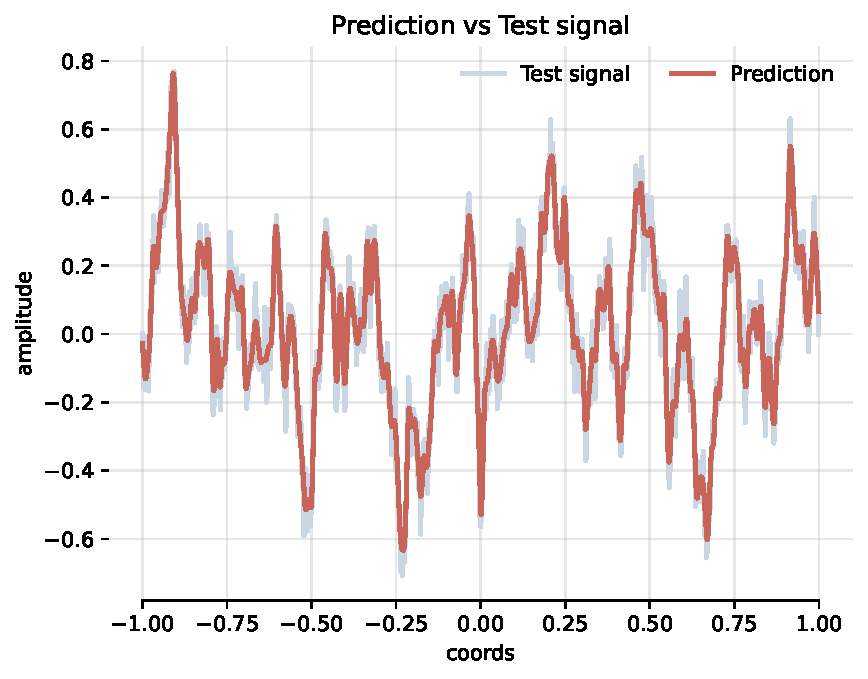
\includegraphics[width=\textwidth]{img/ch3/pred-noise-1hl-32hf-w8.pdf}
        \caption{}
        \label{fig:pred-noise-1hl-32hf-w8}
    \end{subfigure}
    \begin{subfigure}[b]{0.32\textwidth}
        \centering
        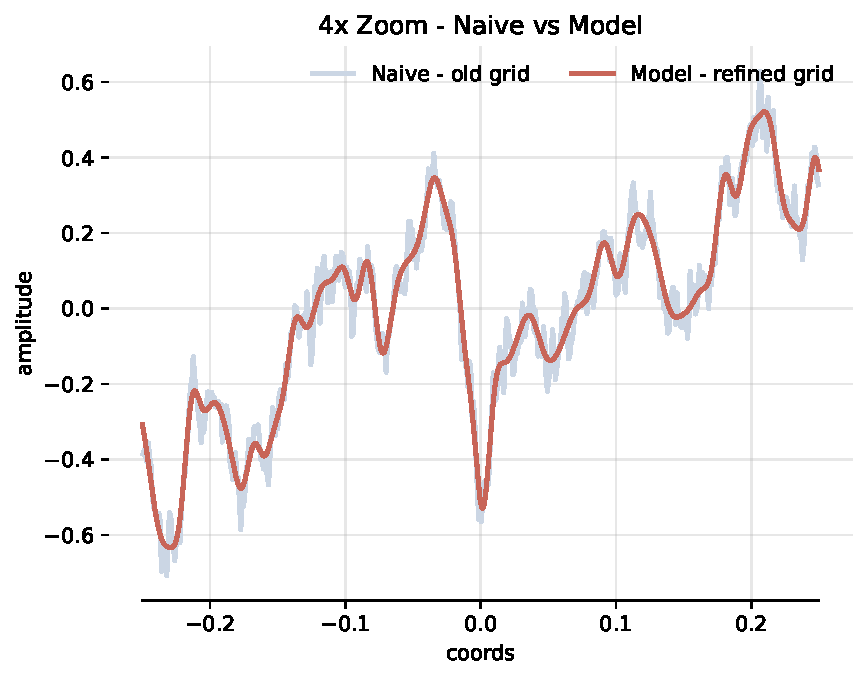
\includegraphics[width=\textwidth]{img/ch3/4x-zoom-noise-1hl-32hf-w8.pdf}
        \caption{}
        \label{fig:4x-zoom-noise-1hl-32hf-w8}
    \end{subfigure}
    \begin{subfigure}[b]{0.32\textwidth}
        \centering
        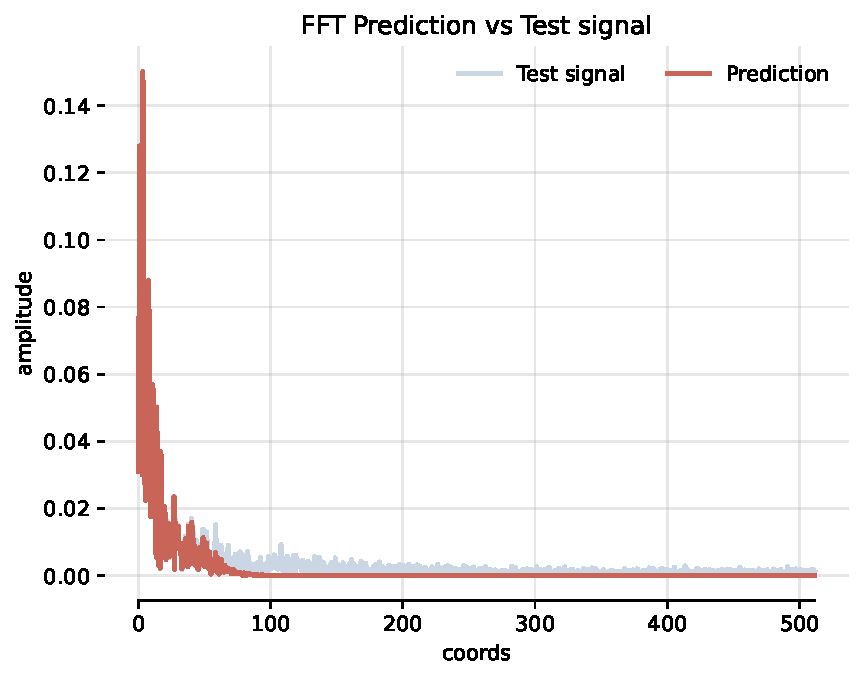
\includegraphics[width=\textwidth]{img/ch3/fft-noise-1hl-32hf-w8.pdf}
        \caption{}
        \label{fig:fft-noise-1hl-32hf-w8}
    \end{subfigure}
    \caption{Smoothed reconstruction with 1 hidden layer}
    \label{f:rec-1hl-32hf-8hz}
\end{figure}

The result in Figure \ref{fig:pred-noise-1hl-32hf-w8} resembles a smoothed version of the input signal, as expected, which is more evident in the zoomed-in view (Figure \ref{fig:4x-zoom-noise-1hl-32hf-w8}). However, the Fast Fourier Transform in Figure \ref{fig:fft-noise-1hl-32hf-w8} shows frequencies much higher than 8 Hz, in contrast to the shallow network experiments shown in Figures \ref{fig:rec-noise-shallow-w8} and \ref{fig:fft-noise-shallow-w8}. The FFT of the reconstructed signal aligns with that of the original signal up to around 30 Hz but fails to capture frequencies precisely within the range up to 100 Hz. Moreover, it does not show contributions from frequencies higher than 100 Hz.

Decreasing the number of neurons per layer slightly reduces the highest frequencies learned by the network, while increasing the network width allows it to capture higher frequencies, as demonstrated in Figure \ref{f:comparison-16-32-64-hf}. This can be observed in the FFT plots (Figures \ref{fig:fft-noise-1hl-16hf-w8}, \ref{fig:fft-noise-1hl-32hf-w8} and \ref{fig:fft-noise-1hl-64hf-w8}), and can also be perceived in the most refined details in the spatial reconstruction of the signal (Figures \ref{fig:4x-zoom-noise-1hl-16hf-w8}, \ref{fig:comp-4x-zoom-noise-1hl-32hf-w8} and \ref{fig:4x-zoom-pred-noise-1hl-64hf-w8}).

\begin{figure}[!h]
    \centering
    \begin{subfigure}[b]{0.32\textwidth}
        \centering
        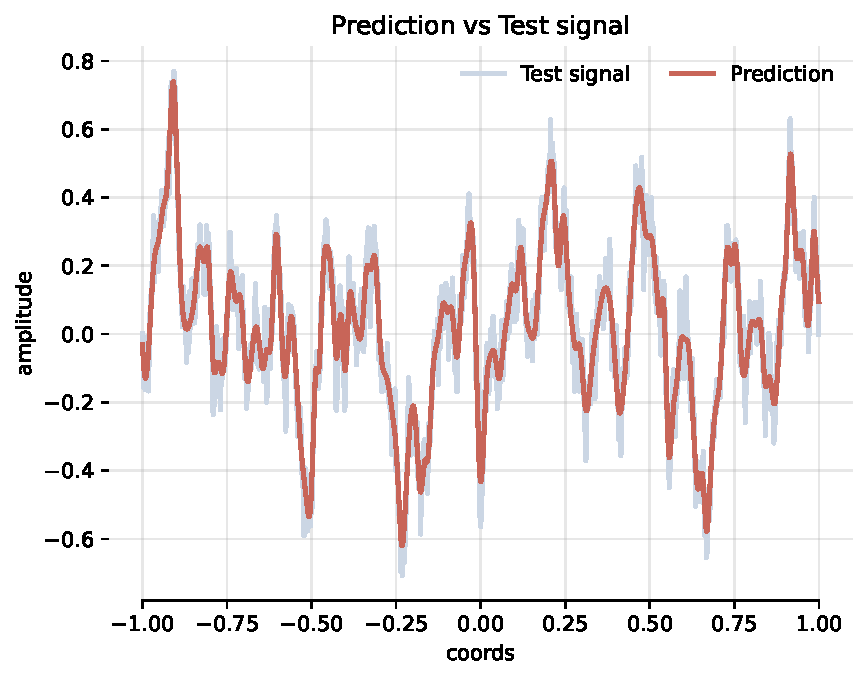
\includegraphics[width=\textwidth]{img/ch3/pred-noise-1hl-16hf-w8.pdf}
        \caption{16 neurons}
        \label{fig:pred-noise-1hl-16hf-w8}
    \end{subfigure}
    \begin{subfigure}[b]{0.32\textwidth}
        \centering
        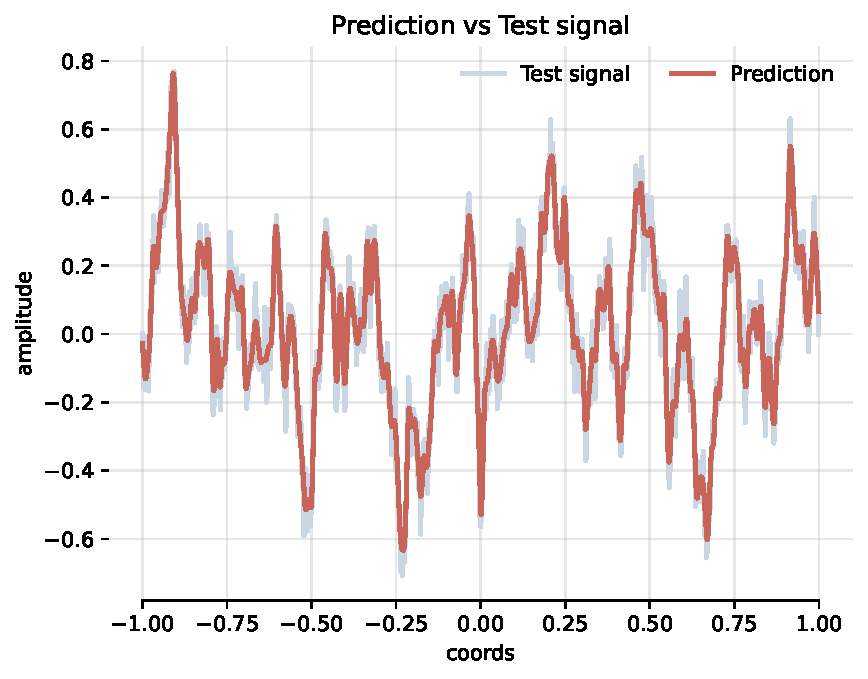
\includegraphics[width=\textwidth]{img/ch3/pred-noise-1hl-32hf-w8.pdf}
        \caption{32 neurons}
        \label{fig:comp-pred-noise-1hl-32hf-w8}
    \end{subfigure}
    \begin{subfigure}[b]{0.32\textwidth}
        \centering
        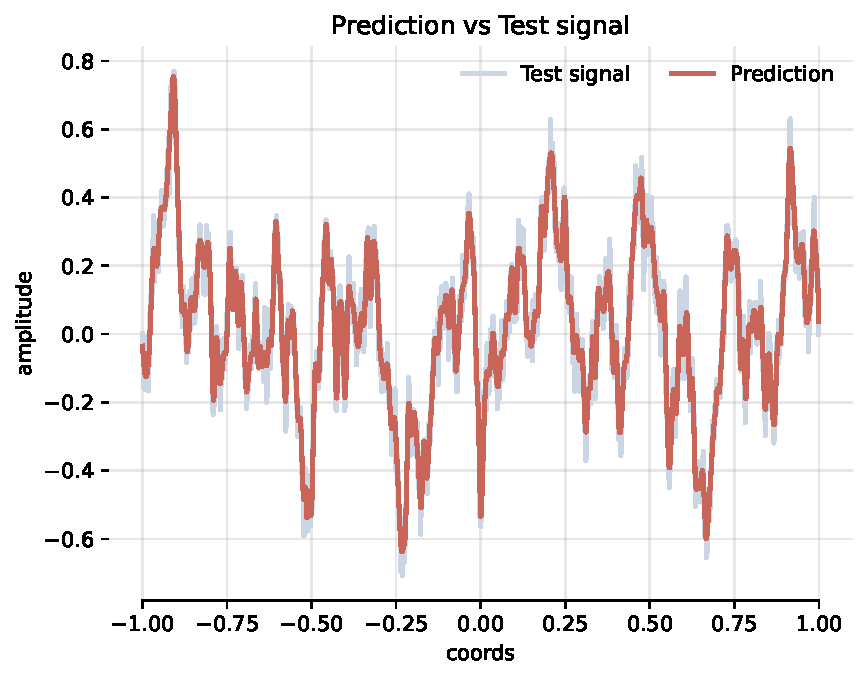
\includegraphics[width=\textwidth]{img/ch3/pred-noise-1hl-64hf-w8.pdf}
        \caption{64 neurons}
        \label{fig:pred-noise-1hl-64hf-w8}
    \end{subfigure}

    \begin{subfigure}[b]{0.32\textwidth}
        \centering
        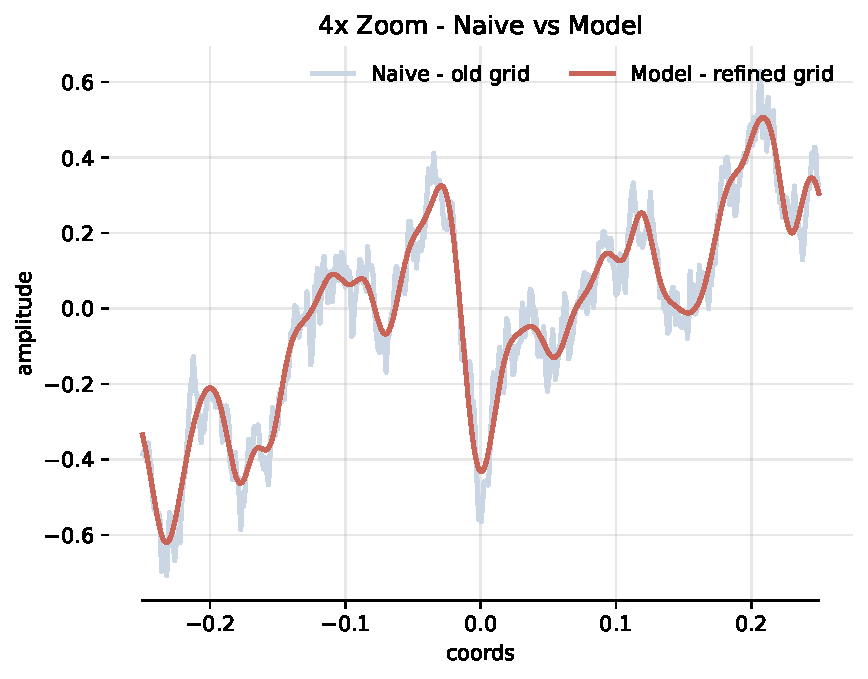
\includegraphics[width=\textwidth]{img/ch3/4x-zoom-noise-1hl-16hf-w8.pdf}
        \caption{16 neurons}
        \label{fig:4x-zoom-noise-1hl-16hf-w8}
    \end{subfigure}
    \begin{subfigure}[b]{0.32\textwidth}
        \centering
        \includegraphics[width=\textwidth]{img/ch3/4x-zoom-noise-1hl-32hf-w8.pdf}
        \caption{32 neurons}
        \label{fig:comp-4x-zoom-noise-1hl-32hf-w8}
    \end{subfigure}
    \begin{subfigure}[b]{0.32\textwidth}
        \centering
        \includegraphics[width=\textwidth]{img/ch3/4x-zoom-noise-1hl-64hf-w8.pdf}
        \caption{64 neurons}
        \label{fig:4x-zoom-pred-noise-1hl-64hf-w8}
    \end{subfigure}

    \begin{subfigure}[b]{0.32\textwidth}
        \centering
        \includegraphics[width=\textwidth]{img/ch3/fft-noise-1hl-16hf-w8.pdf}
        \caption{16 neurons}
        \label{fig:fft-noise-1hl-16hf-w8}
    \end{subfigure}
    \begin{subfigure}[b]{0.32\textwidth}
        \centering
        \includegraphics[width=\textwidth]{img/ch3/fft-noise-1hl-32hf-w8.pdf}
        \caption{32 neurons}
        \label{fig:comp-fft-noise-1hl-32hf-w8}
    \end{subfigure}
    \begin{subfigure}[b]{0.32\textwidth}
        \centering
        \includegraphics[width=\textwidth]{img/ch3/fft-noise-1hl-64hf-w8.pdf}
        \caption{64 neurons}
        \label{fig:fft-noise-1hl-64hf-w8}
    \end{subfigure}
    \caption{Comparison between different network widths}
    \label{f:comparison-16-32-64-hf}
\end{figure}

If we keep the width of the network fixed and increase the range of frequencies used in the initialization, the network can gradually capture higher frequencies. This continues until the network reaches its capacity, after which performance degrades, and the output turns into noise. Figure \ref{f:comparison-8-to-256-hz} illustrates this phenomenon with a network of 32 neurons per layer. Notice that from 8 Hz to 64 Hz, the network gets better in capturing finer details of the signal. However, when $\omega_0=128$, the reconstruction presents peaks and valleys bigger than those present in the signal, an indicative of spurious frequencies. By $\omega_0=256$, the result totally degenerates into noise.

\begin{figure}[h]
    \centering
    \begin{subfigure}[b]{0.32\textwidth}
        \centering
        \includegraphics[width=\textwidth]{img/ch3/16x-zoom-1hl-32hf-8hz.pdf}
        \caption{$\omega_0=8$}
        \label{fig:16x-zoom-1hl-32hf-8hz}
    \end{subfigure}
    \begin{subfigure}[b]{0.32\textwidth}
        \centering
        \includegraphics[width=\textwidth]{img/ch3/16x-zoom-1hl-32hf-16hz.pdf}
        \caption{$\omega_0=16$}
        \label{fig:16x-zoom-1hl-32hf-16hz}
    \end{subfigure}
    \begin{subfigure}[b]{0.32\textwidth}
        \centering
        \includegraphics[width=\textwidth]{img/ch3/16x-zoom-1hl-32hf-32hz.pdf}
        \caption{$\omega_0=32$}
        \label{fig:16x-zoom-1hl-32hf-32hz}
    \end{subfigure}

    \begin{subfigure}[b]{0.32\textwidth}
        \centering
        \includegraphics[width=\textwidth]{img/ch3/16x-zoom-1hl-32hf-64hz.pdf}
        \caption{$\omega_0=64$}
        \label{fig:16x-zoom-1hl-32hf-64hz}
    \end{subfigure}
    \begin{subfigure}[b]{0.32\textwidth}
        \centering
        \includegraphics[width=\textwidth]{img/ch3/16x-zoom-1hl-32hf-128hz.pdf}
        \caption{$\omega_0=128$}
        \label{fig:16x-zoom-1hl-32hf-128hz}
    \end{subfigure}
    \begin{subfigure}[b]{0.32\textwidth}
        \centering
        \includegraphics[width=\textwidth]{img/ch3/16x-zoom-1hl-32hf-256hz.pdf}
        \caption{$\omega_0=256$}
        \label{fig:16x-zoom-1hl-32hf-256hz}
    \end{subfigure}
    \caption{Comparison between different ranges of frequencies in initialization}
    \label{f:comparison-8-to-256-hz}
\end{figure}


% We observe that as we increase the value of $\omega_0$, meaning the frequency interval used in initialization of the first layer of the sinusoidal network, it becomes better in fitting fine details of the signal. Figure \ref{f:zoomed-views-noise} shows some zoomed views of the reconstruction. The grid where the network has been evaluated \red{has been refined XX, XXX and XXXX times}. Note that the model is well behaved in the points that were not given as supervision (not part of the training data), that is, it correctly interpolates the signal.


% On the other hand, if $\omega_0$ is too high it may cause the training to diverge. \red{In the Figure \ref{f:diverging-omega0}, we show the evolution of the training loss (Figure \ref{fig:diverging-loss}) and the result (Figure \ref{fig:diverging-reconstruction}) after 200 epochs when we initialized the SIREN with $\omega_0=600$. Note that after about 50 epochs, the loss starts to increase and our final result bears no resemblance to the original signal.}

\red{We conclude that the frequency initialization of the first layer, which depends on $\omega_0$, is of central importance in the convergence of network training and multiresolution learning. Ideally we should initialize the network with frequencies that match the frequency content of the target signal. However, as we do not have access to this information in many applications, we must guess a value for $\omega_0$. Here, the Shannon-Nyquist therorem may help us bound the value of $\omega_0$. For example, considering a sampling rate of 1024 Hz, we cannot represent frequencies higher than 512 (half the sampling rate), so it does not make sense to choose $\omega_0$ higher than this value. Also, since the composition of sines generates higher frequencies \cite{novello2022understanding}, it is reasonable to initialize the network with much lower frequencies than the Nyquist limit, and the experiments corroborate that.

Another point worth noticing is that if the initialization frequencies are too high, the hidden layers may generate even higher frequencies, and even a model with high capacity will introducing noise into the model's reconstruction. This noise is not evident at the training coodinates, as the model overfits this data well, but it can be observed in a more refined grid FIGURE XXXX.}

% \pagebreak

\subsection{Capacity Filtering}

The experiment illustrated in Figure \ref{f:comparison-16-32-64-hf} suggests that a network's capacity can serve as a filter when learning a signal. To further investigate this behavior, we compared the reconstruction of a stochastic signal using two networks: one with 16 neurons per layer and another with 256 neurons per layer. For this experiment, we generated a new Perlin noise signal with the following parameters: scale = 10, octaves = 14, and persistence = 1.5. Both networks have a single hidden layer and were initialized with $\omega_0=2$ Hz. The results are shown in Figure \ref{f:capacity-filter-16-hf-256}. 

\begin{figure}[h]
    \centering
    \begin{subfigure}[b]{0.32\textwidth}
        \centering
        \includegraphics[width=\textwidth]{img/ch3/pred-1hl-16hf-2hz.pdf}
        \caption{16 neurons}
        \label{fig:pred-1hl-16hf-2hz}
    \end{subfigure}
    \begin{subfigure}[b]{0.32\textwidth}
        \centering
        \includegraphics[width=\textwidth]{img/ch3/16x-zoom-1hl-16hf-2hz.pdf}
        \caption{16 neurons}
        \label{fig:16x-zoom-1hl-16hf-2hz}
    \end{subfigure}
    \begin{subfigure}[b]{0.32\textwidth}
        \centering
        \includegraphics[width=\textwidth]{img/ch3/fft-1hl-16hf-2hz.pdf}
        \caption{16 neurons}
        \label{fig:fft-1hl-16hf-2hz}
    \end{subfigure}

    \begin{subfigure}[b]{0.32\textwidth}
        \centering
        \includegraphics[width=\textwidth]{img/ch3/pred-1hl-256hf-2hz.pdf}
        \caption{256 neurons}
        \label{fig:pred-1hl-256hf-2hz}
    \end{subfigure}
    \begin{subfigure}[b]{0.32\textwidth}
        \centering
        \includegraphics[width=\textwidth]{img/ch3/16x-zoom-1hl-256hf-2hz.pdf}
        \caption{256 neurons}
        \label{fig:16x-zoom-1hl-256hf-2hz}
    \end{subfigure}
    \begin{subfigure}[b]{0.32\textwidth}
        \centering
        \includegraphics[width=\textwidth]{img/ch3/fft-1hl-256hf-2hz.pdf}
        \caption{256 neurons}
        \label{fig:fft-1hl-256hf-2hz}
    \end{subfigure}
    \caption{Comparison of reconstructions using networks with a single hidden layer and varying capacities.}
    \label{f:capacity-filter-16-hf-256}
\end{figure}

As expected, both networks produce smoothed versions of the input signal due to their initialization with low frequencies. However, the smaller network (top row) produces a significantly smoother reconstruction compared to the larger network (bottom row). This observation can be attributed to the smaller capacity of the network, which restricts it from learning higher frequencies. This highlights the role of network capacity as a natural frequency filter.

Previous work by \cite{Rahaman2018O} has demonstrated that during training, a Multi-Layer Perceptron (MLP) tends to learn lower frequencies before higher ones, a phenomenon known as spectral bias. Because sinusoidal neural networks are a form of MLP, this explains why, for a fixed depth, the network's width can act as a frequency filter. This capacity-based filtering effect, however, only holds if the network has sufficient capacity to capture the lower frequencies in the signal. As we increase the value of $\omega_0$ to capture higher frequencies, the network with 16 neurons per layer eventually becomes unable to fit the signal, and the reconstruction quality deteriorates. Figure \ref{f:capacity-filter-16hf-increasing-omega} provides zoomed-in views of reconstructions using a network with 16 neurons per layer initialized with different values of $\omega_0$. Notice how the reconstruction becomes progressively more detailed and closer to the input signal as $\omega_0$ increases, up to $\omega_0 = 32$. However, at $\omega_0=64$, the result degrades significantly.

\begin{figure}[h]
    \centering
    \begin{subfigure}[b]{0.32\textwidth}
        \centering
        \includegraphics[width=\textwidth]{img/ch3/16x-zoom-1hl-16hf-2hz.pdf}
        \caption{$\omega_0=2$ Hz}
        % \label{fig:pred-1hl-16hf-2hz}
    \end{subfigure}
    \begin{subfigure}[b]{0.32\textwidth}
        \centering
        \includegraphics[width=\textwidth]{img/ch3/16x_zoom-1hl-16hf-4hz.pdf}
        \caption{$\omega_0=4$ Hz}
        % \label{fig:16x-zoom-1hl-16hf-2hz}
    \end{subfigure}
    \begin{subfigure}[b]{0.32\textwidth}
        \centering
        \includegraphics[width=\textwidth]{img/ch3/16x_zoom-1hl-16hf-8hz.pdf}
        \caption{$\omega_0=8$ Hz}
        % \label{fig:fft-1hl-16hf-2hz}
    \end{subfigure}

    \begin{subfigure}[b]{0.32\textwidth}
        \centering
        \includegraphics[width=\textwidth]{img/ch3/16x_zoom-1hl-16hf-16hz.pdf}
        \caption{$\omega_0=16$ Hz}
        % \label{fig:pred-1hl-256hf-2hz}
    \end{subfigure}
    \begin{subfigure}[b]{0.32\textwidth}
        \centering
        \includegraphics[width=\textwidth]{img/ch3/16x_zoom-1hl-16hf-32hz.pdf}
        \caption{$\omega_0=32$ Hz}
        % \label{fig:16x-zoom-1hl-256hf-2hz}
    \end{subfigure}
    \begin{subfigure}[b]{0.32\textwidth}
        \centering
        \includegraphics[width=\textwidth]{img/ch3/16x_zoom-1hl-16hf-64hz.pdf}
        \caption{$\omega_0=64$ Hz}
        % \label{fig:pred-1hl-16hf-64hz}
    \end{subfigure}
    \caption{Comparison of reconstructions using a small network with varying values of $\omega_0$.}
    \label{f:capacity-filter-16hf-increasing-omega}
\end{figure}

\section{Training, Generalization and Representation}

% \red{We have established that we can bound the frequencies learned by a sinusoidal neural network by adjusting the interval of frequencies sampled for initialization of its first layer, and also by adjusting the network capacity. That is, if the value of $\omega_0$ is too low, the network will learn the lower frequencies of the signal, fitting their intensities in the Fourier spectrum, but won't learn the higher frequencies, even if it has enough computational units to to do. On the other hand, if the capacity given by the computational units is too small, the result will also resemble a filtered version of the target signal. TALVEZ MOVER PARA O CHAPTER 4 - MR-TRAINING}

Neural networks have been extensively used as analysis tools, as models trained in large datasets to recognize patterns and construct features to specific data types. However, we are using coordinate-based neural networks to represent signals. Our dataset is only 1 signal, or better saying, it is a set of samples of this signal, for example, a discrete set of coordinates and values. 

Some people say \red{trazer referências} that this is equivalennt to overfit a neural network to the signal, but we do not think this is the appropriate way to frame the problem. We want the neural network to be a continuous representation of a signal for which we only know a limited amount of samples. We actually need to solve a problem of  sampling and reconstruction, a classical problem in signal processing, guaranteeing that the neural representation contains the samples but also that it is "well behaved" in between. That means that when thinking of overfitting and generalization, we should borrow the perspective of regression problems and interpolation. For example, in polynomial interpolation it is known that high-degree polynomials will oscilate a lot, inclusing in regions between the interpolated points.

In this section, we investigate how well sinusoidal neural networks generalize to represent signals. To this end, we run experiments trying to reconstruct a signal from a critically sampled representation. For this, we take an input signal and we compute its Gaussian pyramid representation, that is, we filter the signal with a low-pass filter and subsample it by a factor of 2, repeating this procedure several times. We use these subsampled signals as training data for our experiments. 

On the other hand, additionally, we build a Gaussian Tower, that is, a filtered representation without decimation. To compensate for the lack of subsampling, we double the window of the filter for each level of the tower. This way, for a signal like a high frequency Perlin noise, the original signal is critically sampled, but the other levels of the Gaussian Tower are oversampled. According to the signal processing theory, for each level, it should be possible to perfectly reconstruct teh signal using only the samples in the Gaussian Pyramid. This way, we train the network in a Gaussian pyramid signal and we evaluate it against its correspondent in the Gaussian Tower. By sampling the network in a much more refined grid, and having a baseline to compare, we can verify if it is accuratelly representing the signal or if it is overfitting, that is, learning how to perfectly fit the samples, but introducing spurious frequencies and oscilating in between the supervised points.

For the next experiments, we generate another Perlin noise with the following parameters: scale: 10; octaves: 8; persistence: 0.9.



% - Present the experiments in fitting multiresolution signals
%     - 1D Gaussian Tower
%     - 1D Gaussian Pyramid
%     - show that networks is well behaved between samples

% \subsection{Gaussian Pyramid Training}


% After exploring the impact of different values of initialization frequencies, we investigated if we could fit multiple scales of the same signal by building a Gaussian pyramid of it. We filtered the signal using a box filter of dimension 5, decimated it by a factor of 2 and used this subsampled version to train our network. Then, we used the trained network to predict the values over all originally sampled points, so we could verify its behaviour on unsupervised points. As we are filtering the higher frequencies of the signal, we expect to be able to represent it exactly by using fewer samples, acconding to the classical sampling theory.  
% We compared our result to a smoothed but not decimated version of the signal where we doubled the size of the filter as we walked to coarse scales. The panel of figures below shows the result of fitting a signal in 7 different scales, starting with \omega_0=256 and dividing it by 2 as we walk to coarse scales.
% We trained the network using less points at each scale.

% \begin{figure}[!htb]
% \minipage{0.49\textwidth}
% \includegraphics[width=\linewidth]{charts/Section-20-Panel-0-ulotlhctz}
% \caption{}
% \endminipage\hfill
% \minipage{0.49\textwidth}
% \includegraphics[width=\linewidth]{charts/Section-20-Panel-1-twwld6gku}
% \caption{}
% \endminipage
% \end{figure}


% \chapter{Multiresolution Sinusoidal Neural Networks}
% \label{ch:mrnet}

% In recent years, the computer science community has seen an explosion in research in neural networks, motivated mainly by advances in Deep Learning~\cite{lecun2015deep,goodfellow2016deep}.
% For visual computing, this was spurred by the creation of Convolutional Neural Networks~(CNNs)~\cite{cnn98}, which had a significant impact both for the research community and the society at large~\cite{li2021survey,shamsaldin2019study}.
% The effectiveness of CNNs comes from the translation invariant properties of the convolution operator, which makes it a proper architecture for the analysis of visual imagery.

% Deep neural networks such as CNNs, employ an array-based discrete representation of the underlying signal. In this case, the network input consists of a vector of pixel values (in RGB) representing the image \emph{directly} by data samples. We call this kind of network a \textit{data-based} network.


% Moreover, the revolution in the media industry caused by deep neural networks motivated the development of new image representations using neural networks. While the data-based network is appropriate for analysis tasks, relying on a discretization of the image, another kind of network called \textit{coordinate-based~network} is suitable for synthesis, and provides a continuous and compact representation. For its characteristics, there is a growing interest in using these networks in imaging applications~\cite{xie2022neural}.
% For instance, coordinate-based networks have been successfully applied in image compression~\cite{dupont2021coin} and super-resolution~\cite{czerkawski2021neural}.


% A coordinate-based network represents the image \emph{indirectly} using a fully connected \textit{multi-layer perceptron} (MLP) that takes as input a pixel coordinate and outputs a RGB color. These~networks provide a continuous implicit representation for images~\cite{chen2021learning}, and allow for various applications, from Neural Signed Distance Functions~(NeuralSDFs)~\cite{park2019deepsdf} to Neural Radiance Fields~(NeRFs)~\cite{mildenhall2021nerf}. Since the coordinates are continuous, images can be presented in arbitrary resolution.

% % Sinusoidal neural networks are particularly suited to model stationary or quasi-stationary signals due to the periodic nature of its activation function~\cite{chen2022}.

% Sinusoidal neural networks are examples of coordinate-based networks in which their activation function is the sine function. As such, they bridge the gap between the spatial and spectral domains, given the close relationship of the sine function with the Fourier~basis. However, these sinusoidal neural networks have been regarded as difficult to train~\cite{taming2017}. To overcome this problem, \citet{sitzmann2019siren} proposed a sinusoidal network for signal representation called SIREN. One of the key contributions of this work is the initialization scheme that guarantees stability and good convergence. Furthermore, it also allows modeling fine details in accordance with the signal’s frequency content.

% A \textit{multiplicative filter network} (MFN) is a sinusoidal network simpler than SIREN which is equivalent to a shallow sinusoidal network~\cite{fathony2020multiplicative}. \citet{bacon2021} presented \textit{band-limited coordinate network }(BACON), an MFN that produces intermediate outputs with an analytical spectral bandwidth (specified at initialization) and achieves multiresolution of the underlying signal. While its structure allows BACON to be expressed as a linear combinations of sines, avoiding the composition of sines present in sinusoidal MLPs, it creates multiresolution representations by truncating the frequency spectra of the signals. This approach produces ringing artifacts  in some levels of detail, and becomes evident when we look at the Fourier transform of the images.

% The control of frequency bands in the representation is closely related with the capability of adaptive reconstruction of the signal in multiple levels of detail.
% In that context, \citet{mueller2022instant} developed a multiresolution neural network architecture based on hash encoding. Also, \citet{martel2021acorn} designed an adaptive coordinate network for neural signals.

% In this context, we introduce \textit{multiresolution sinusoidal neural networks}~(MR-Net) based on classical signal multiresolution representations. 
% Our results, presented in Section~\ref{sub:spectra-eval}, indicate that using MR-Net produces better results compared to the previous state-of-the-art technique, BACON, while employing a smaller number of parameters.
% We describe three MR-Net subclasses: S-Net, L-Net and M-Net.
% Finally, we present applications on antialiasing and level-of-detail reconstruction.

% - Related Works: Mip-Nerf; Bacon; 